Most every practical digital modulation uses a finite symbol alphabet instead of a continuous transmit distribution.
In our formalism this means that $i$ is chosen from an alphabet $i \in \SymbolAlphabet$, $\SymbolAlphabet = \{ s_1 , \ldots , s_M \} \subset \Disk$,
associated with $z \in \SymbolAlphabetZL$ from a load impedance alphabet $\SymbolAlphabetZL = \ChannelFunc^{-1}(\SymbolAlphabet) = \{ z_1 , \ldots , z_M \} \subset \HalfPlane$.
This caps the achievable rate at $\log_2(M)$ bpcu.
The Euclidean symbol distance $|s_m - s_n| \leq 2\DiskRadius$ is capped by the disk diameter.
This maximum is attained by a binary alphabet 
$\SymbolAlphabet = \{ 0, 2\DiskRadius \}$,
$\SymbolAlphabetZL = \{ \infty , 0\}$
but also by
$\SymbolAlphabet = \{ \DiskRadius(1+j) , \DiskRadius(1-j) \}$,
$\SymbolAlphabetZL = \{ -j , +j \}$
or any rotation of such $\SymbolAlphabet$ about $\DiskRadius$.

$M$-ary phase shift keying ($M$-PSK) is a more capable alphabet. It uses $M = 2^\ell$ symbols %($\ell \in \bbN$)
at $s_m = \DiskRadius(1+\exp(j2\pi\f{m - 1/2}{M}))$.
As mentioned earlier, this modulation is realized with a purely reactive load circuit.
\Cref{fig:Constellation_rate} shows the achievable rate of various PSK schemes. %with soft decoding (i.e. based on the unquantized observation $y$). 
The underlying numerical rate computation is described in \Cref{apdx:ar}.
At low SNR, $M$-PSK with $M \geq 4$ yields data rates very close to channel capacity while uniform-PSK ($M = \infty$) even achieves capacity.

\begin{figure}[!ht]
\centering
\vspace{-5mm}
\subfloat[symbol alphabet, TX current]{%
\resizebox{!}{60mm}{% This file was created by matlab2tikz.
%
%The latest updates can be retrieved from
%  http://www.mathworks.com/matlabcentral/fileexchange/22022-matlab2tikz-matlab2tikz
%where you can also make suggestions and rate matlab2tikz.
%
\definecolor{magenta}{rgb}{1.00000,0.00000,1.00000}%
%
\begin{tikzpicture}[>=latex']

\begin{axis}[%
width=1.6185in,
height=2.0601in,
at={(0,0)},
scale only axis,
xmin=-0.1,
xmax=2.1,
xlabel style={font=\color{white!15!black},at={(0.48,-0.065)},anchor=north},
xlabel={$\Re(i) \, / \, \DiskRadius$},
ymin=-1.4,
ymax=1.4,
ylabel style={font=\color{white!15!black},at={(-0.065,0.585)}},
ylabel={$\Im(i) \, / \, \DiskRadius$},
xtick={0,1,2},
ytick={-1,0,1},
axis background/.style={fill=white},
xmajorgrids,
ymajorgrids,
legend style={legend cell align=left, align=left, draw=white!15!black}
]
\addplot [color=white!85!black, forget plot]
  table[row sep=crcr]{%
2	0\\
1.9993908270191	0.034899496702501\\
1.99756405025982	0.0697564737441253\\
1.99452189536827	0.104528463267653\\
1.99026806874157	0.139173100960065\\
1.98480775301221	0.17364817766693\\
1.97814760073381	0.207911690817759\\
1.970295726276	0.241921895599668\\
1.96126169593832	0.275637355816999\\
1.95105651629515	0.309016994374947\\
1.93969262078591	0.342020143325669\\
1.92718385456679	0.374606593415912\\
1.9135454576426	0.4067366430758\\
1.89879404629917	0.438371146789077\\
1.88294759285893	0.469471562785891\\
1.86602540378444	0.5\\
1.84804809615643	0.529919264233205\\
1.82903757255504	0.559192903470747\\
1.80901699437495	0.587785252292473\\
1.78801075360672	0.615661475325658\\
1.76604444311898	0.642787609686539\\
1.74314482547739	0.669130606358858\\
1.71933980033865	0.694658370458997\\
1.694658370459	0.719339800338651\\
1.66913060635886	0.743144825477394\\
1.64278760968654	0.766044443118978\\
1.61566147532566	0.788010753606722\\
1.58778525229247	0.809016994374947\\
1.55919290347075	0.829037572555042\\
1.5299192642332	0.848048096156426\\
1.5	0.866025403784439\\
1.46947156278589	0.882947592858927\\
1.43837114678908	0.898794046299167\\
1.4067366430758	0.913545457642601\\
1.37460659341591	0.927183854566787\\
1.34202014332567	0.939692620785908\\
1.30901699437495	0.951056516295154\\
1.275637355817	0.961261695938319\\
1.24192189559967	0.970295726275996\\
1.20791169081776	0.978147600733806\\
1.17364817766693	0.984807753012208\\
1.13917310096007	0.99026806874157\\
1.10452846326765	0.994521895368273\\
1.06975647374413	0.997564050259824\\
1.0348994967025	0.999390827019096\\
1	1\\
0.965100503297499	0.999390827019096\\
0.930243526255875	0.997564050259824\\
0.895471536732347	0.994521895368273\\
0.860826899039935	0.99026806874157\\
0.82635182233307	0.984807753012208\\
0.792088309182241	0.978147600733806\\
0.758078104400332	0.970295726275996\\
0.724362644183001	0.961261695938319\\
0.690983005625053	0.951056516295154\\
0.657979856674331	0.939692620785908\\
0.625393406584088	0.927183854566787\\
0.5932633569242	0.913545457642601\\
0.561628853210922	0.898794046299167\\
0.530528437214109	0.882947592858927\\
0.5	0.866025403784439\\
0.470080735766795	0.848048096156426\\
0.440807096529253	0.829037572555042\\
0.412214747707527	0.809016994374947\\
0.384338524674342	0.788010753606722\\
0.357212390313461	0.766044443118978\\
0.330869393641142	0.743144825477394\\
0.305341629541003	0.719339800338651\\
0.280660199661349	0.694658370458997\\
0.256855174522606	0.669130606358858\\
0.233955556881022	0.642787609686539\\
0.211989246393278	0.615661475325658\\
0.190983005625053	0.587785252292473\\
0.170962427444958	0.559192903470747\\
0.151951903843574	0.529919264233205\\
0.133974596215561	0.5\\
0.117052407141073	0.469471562785891\\
0.101205953700833	0.438371146789077\\
0.0864545423573992	0.4067366430758\\
0.0728161454332127	0.374606593415912\\
0.0603073792140917	0.342020143325669\\
0.0489434837048465	0.309016994374948\\
0.0387383040616813	0.275637355817\\
0.0297042737240035	0.241921895599668\\
0.0218523992661943	0.207911690817759\\
0.015192246987792	0.17364817766693\\
0.00973193125842975	0.139173100960066\\
0.00547810463172671	0.104528463267654\\
0.0024359497401758	0.0697564737441255\\
0.000609172980904238	0.0348994967025007\\
0	1.22464679914735e-16\\
0.000609172980904238	-0.0348994967025009\\
0.00243594974017569	-0.0697564737441248\\
0.0054781046317266	-0.104528463267653\\
0.00973193125842975	-0.139173100960066\\
0.015192246987792	-0.17364817766693\\
0.0218523992661943	-0.207911690817759\\
0.0297042737240034	-0.241921895599668\\
0.0387383040616811	-0.275637355816999\\
0.0489434837048465	-0.309016994374948\\
0.0603073792140916	-0.342020143325669\\
0.0728161454332126	-0.374606593415912\\
0.0864545423573989	-0.4067366430758\\
0.101205953700833	-0.438371146789077\\
0.117052407141073	-0.469471562785891\\
0.133974596215561	-0.5\\
0.151951903843574	-0.529919264233205\\
0.170962427444958	-0.559192903470747\\
0.190983005625053	-0.587785252292473\\
0.211989246393278	-0.615661475325658\\
0.233955556881022	-0.642787609686539\\
0.256855174522606	-0.669130606358858\\
0.280660199661349	-0.694658370458997\\
0.305341629541003	-0.719339800338651\\
0.330869393641142	-0.743144825477394\\
0.357212390313461	-0.766044443118978\\
0.384338524674342	-0.788010753606722\\
0.412214747707527	-0.809016994374947\\
0.440807096529253	-0.829037572555041\\
0.470080735766795	-0.848048096156426\\
0.5	-0.866025403784438\\
0.530528437214109	-0.882947592858927\\
0.561628853210922	-0.898794046299167\\
0.5932633569242	-0.913545457642601\\
0.625393406584088	-0.927183854566787\\
0.657979856674331	-0.939692620785908\\
0.690983005625052	-0.951056516295154\\
0.724362644183001	-0.961261695938319\\
0.758078104400332	-0.970295726275996\\
0.79208830918224	-0.978147600733806\\
0.82635182233307	-0.984807753012208\\
0.860826899039935	-0.99026806874157\\
0.895471536732347	-0.994521895368273\\
0.930243526255874	-0.997564050259824\\
0.965100503297498	-0.999390827019096\\
1	-1\\
1.0348994967025	-0.999390827019096\\
1.06975647374413	-0.997564050259824\\
1.10452846326765	-0.994521895368273\\
1.13917310096007	-0.99026806874157\\
1.17364817766693	-0.984807753012208\\
1.20791169081776	-0.978147600733806\\
1.24192189559967	-0.970295726275997\\
1.275637355817	-0.961261695938319\\
1.30901699437495	-0.951056516295154\\
1.34202014332567	-0.939692620785909\\
1.37460659341591	-0.927183854566787\\
1.4067366430758	-0.913545457642601\\
1.43837114678908	-0.898794046299167\\
1.46947156278589	-0.882947592858927\\
1.5	-0.866025403784439\\
1.5299192642332	-0.848048096156426\\
1.55919290347075	-0.829037572555042\\
1.58778525229247	-0.809016994374948\\
1.61566147532566	-0.788010753606722\\
1.64278760968654	-0.766044443118978\\
1.66913060635886	-0.743144825477395\\
1.694658370459	-0.719339800338652\\
1.71933980033865	-0.694658370458998\\
1.74314482547739	-0.669130606358858\\
1.76604444311898	-0.64278760968654\\
1.78801075360672	-0.615661475325659\\
1.80901699437495	-0.587785252292473\\
1.82903757255504	-0.559192903470747\\
1.84804809615643	-0.529919264233206\\
1.86602540378444	-0.5\\
1.88294759285893	-0.469471562785891\\
1.89879404629917	-0.438371146789077\\
1.9135454576426	-0.4067366430758\\
1.92718385456679	-0.374606593415912\\
1.93969262078591	-0.342020143325669\\
1.95105651629515	-0.309016994374948\\
1.96126169593832	-0.275637355817\\
1.970295726276	-0.241921895599668\\
1.97814760073381	-0.20791169081776\\
1.98480775301221	-0.173648177666931\\
1.99026806874157	-0.139173100960066\\
1.99452189536827	-0.104528463267653\\
1.99756405025982	-0.0697564737441248\\
1.9993908270191	-0.0348994967025008\\
2	-2.44929359829471e-16\\
};
\addplot [color=white!85!black, forget plot]
  table[row sep=crcr]{%
1.83	0\\
1.82949438642585	0.0289665822630758\\
1.82797816171565	0.057897873207624\\
1.82545317315567	0.0867586245121524\\
1.8219224970555	0.115513673796854\\
1.81739043500013	0.144127987463552\\
1.81186250860906	0.17256670337874\\
1.80534545280908	0.200795173347724\\
1.7978472076288	0.228779005328109\\
1.78937690852498	0.256484105331206\\
1.7799448752523	0.283876718960305\\
1.76956259929043	0.310923472535207\\
1.75824272984336	0.337591413752914\\
1.74599905842831	0.363848051834934\\
1.73284650207291	0.389661397112289\\
1.71880108514108	0.415\\
1.70387991980983	0.43983298931356\\
1.68810118522068	0.46413010988072\\
1.67148410533121	0.487861759402753\\
1.65404892549358	0.510999024520296\\
1.63581688778875	0.533513716039828\\
1.61681020514624	0.555378403277852\\
1.59705203428108	0.576566447480968\\
1.57656644748097	0.59705203428108\\
1.55537840327785	0.616810205146237\\
1.53351371603983	0.635816887788752\\
1.5109990245203	0.654048925493579\\
1.48786175940275	0.671484105331206\\
1.46413010988072	0.688101185220685\\
1.43983298931356	0.703879919809834\\
1.415	0.718801085141084\\
1.38966139711229	0.732846502072909\\
1.36384805183493	0.745999058428309\\
1.33759141375291	0.758242729843359\\
1.31092347253521	0.769562599290434\\
1.28387671896031	0.779944875252304\\
1.25648410533121	0.789376908524977\\
1.22877900532811	0.797847207628805\\
1.20079517334772	0.805345452809077\\
1.17256670337874	0.811862508609059\\
1.14412798746355	0.817390435000133\\
1.11551367379685	0.821922497055503\\
1.08675862451215	0.825453173155667\\
1.05789787320762	0.827978161715654\\
1.02896658226308	0.829494386425849\\
1	0.83\\
0.971033417736924	0.829494386425849\\
0.942102126792376	0.827978161715654\\
0.913241375487848	0.825453173155667\\
0.884486326203146	0.821922497055503\\
0.855872012536448	0.817390435000133\\
0.82743329662126	0.811862508609059\\
0.799204826652276	0.805345452809077\\
0.771220994671891	0.797847207628805\\
0.743515894668794	0.789376908524977\\
0.716123281039695	0.779944875252304\\
0.689076527464793	0.769562599290434\\
0.662408586247086	0.758242729843359\\
0.636151948165066	0.745999058428308\\
0.610338602887711	0.732846502072909\\
0.585	0.718801085141084\\
0.56016701068644	0.703879919809834\\
0.53586989011928	0.688101185220685\\
0.512138240597247	0.671484105331206\\
0.489000975479704	0.654048925493579\\
0.466486283960172	0.635816887788752\\
0.444621596722148	0.616810205146237\\
0.423433552519032	0.597052034281081\\
0.402947965718919	0.576566447480968\\
0.383189794853763	0.555378403277852\\
0.364183112211248	0.533513716039828\\
0.345951074506421	0.510999024520296\\
0.328515894668794	0.487861759402753\\
0.311898814779315	0.46413010988072\\
0.296120080190166	0.43983298931356\\
0.281198914858916	0.415\\
0.267153497927091	0.38966139711229\\
0.254000941571691	0.363848051834934\\
0.241757270156641	0.337591413752914\\
0.230437400709567	0.310923472535207\\
0.220055124747696	0.283876718960305\\
0.210623091475023	0.256484105331206\\
0.202152792371196	0.22877900532811\\
0.194654547190923	0.200795173347724\\
0.188137491390941	0.17256670337874\\
0.182609564999867	0.144127987463552\\
0.178077502944497	0.115513673796855\\
0.174546826844333	0.0867586245121526\\
0.172021838284346	0.0578978732076242\\
0.170505613574151	0.0289665822630756\\
0.17	1.0164568432923e-16\\
0.170505613574151	-0.0289665822630757\\
0.172021838284346	-0.0578978732076236\\
0.174546826844333	-0.086758624512152\\
0.178077502944497	-0.115513673796854\\
0.182609564999867	-0.144127987463552\\
0.188137491390941	-0.17256670337874\\
0.194654547190923	-0.200795173347724\\
0.202152792371195	-0.228779005328109\\
0.210623091475023	-0.256484105331207\\
0.220055124747696	-0.283876718960305\\
0.230437400709566	-0.310923472535207\\
0.241757270156641	-0.337591413752914\\
0.254000941571691	-0.363848051834934\\
0.267153497927091	-0.389661397112289\\
0.281198914858916	-0.415\\
0.296120080190166	-0.43983298931356\\
0.311898814779315	-0.46413010988072\\
0.328515894668794	-0.487861759402753\\
0.345951074506421	-0.510999024520296\\
0.364183112211248	-0.533513716039828\\
0.383189794853763	-0.555378403277852\\
0.40294796571892	-0.576566447480968\\
0.423433552519032	-0.59705203428108\\
0.444621596722148	-0.616810205146237\\
0.466486283960172	-0.635816887788752\\
0.489000975479704	-0.654048925493579\\
0.512138240597247	-0.671484105331206\\
0.53586989011928	-0.688101185220684\\
0.56016701068644	-0.703879919809834\\
0.585	-0.718801085141084\\
0.610338602887711	-0.732846502072909\\
0.636151948165065	-0.745999058428308\\
0.662408586247086	-0.758242729843359\\
0.689076527464793	-0.769562599290433\\
0.716123281039694	-0.779944875252304\\
0.743515894668794	-0.789376908524977\\
0.771220994671891	-0.797847207628805\\
0.799204826652276	-0.805345452809077\\
0.827433296621259	-0.811862508609059\\
0.855872012536448	-0.817390435000133\\
0.884486326203146	-0.821922497055503\\
0.913241375487848	-0.825453173155667\\
0.942102126792376	-0.827978161715654\\
0.971033417736924	-0.829494386425849\\
1	-0.83\\
1.02896658226308	-0.829494386425849\\
1.05789787320762	-0.827978161715654\\
1.08675862451215	-0.825453173155667\\
1.11551367379685	-0.821922497055503\\
1.14412798746355	-0.817390435000133\\
1.17256670337874	-0.811862508609059\\
1.20079517334772	-0.805345452809077\\
1.22877900532811	-0.797847207628805\\
1.25648410533121	-0.789376908524977\\
1.2838767189603	-0.779944875252304\\
1.31092347253521	-0.769562599290434\\
1.33759141375291	-0.758242729843359\\
1.36384805183493	-0.745999058428309\\
1.38966139711229	-0.732846502072909\\
1.415	-0.718801085141084\\
1.43983298931356	-0.703879919809834\\
1.46413010988072	-0.688101185220685\\
1.48786175940275	-0.671484105331206\\
1.5109990245203	-0.654048925493579\\
1.53351371603983	-0.635816887788752\\
1.55537840327785	-0.616810205146238\\
1.57656644748097	-0.597052034281081\\
1.59705203428108	-0.576566447480968\\
1.61681020514624	-0.555378403277852\\
1.63581688778875	-0.533513716039828\\
1.65404892549358	-0.510999024520297\\
1.67148410533121	-0.487861759402753\\
1.68810118522068	-0.46413010988072\\
1.70387991980983	-0.439832989313561\\
1.71880108514108	-0.415\\
1.73284650207291	-0.389661397112289\\
1.74599905842831	-0.363848051834934\\
1.75824272984336	-0.337591413752914\\
1.76956259929043	-0.310923472535207\\
1.7799448752523	-0.283876718960305\\
1.78937690852498	-0.256484105331207\\
1.7978472076288	-0.22877900532811\\
1.80534545280908	-0.200795173347724\\
1.81186250860906	-0.172566703378741\\
1.81739043500013	-0.144127987463553\\
1.8219224970555	-0.115513673796855\\
1.82545317315567	-0.0867586245121523\\
1.82797816171565	-0.0578978732076235\\
1.82949438642585	-0.0289665822630757\\
1.83	-2.03291368658461e-16\\
};
\addplot [color=white!85!black, forget plot]
  table[row sep=crcr]{%
1.7	0\\
1.69957357891337	0.0244296476917507\\
1.69829483518188	0.0488295316208877\\
1.69616532675779	0.0731699242873574\\
1.6931876481191	0.0974211706720458\\
1.68936542710855	0.121553724366851\\
1.68470332051366	0.145538183572432\\
1.6792070083932	0.169345326919767\\
1.67288318715682	0.192946149071899\\
1.66573956140661	0.216311896062463\\
1.65778483455014	0.239414100327968\\
1.64902869819675	0.262224615391138\\
1.63948182034982	0.28471565015306\\
1.62915583240942	0.306859802752354\\
1.61806331500125	0.328630093950124\\
1.60621778264911	0.35\\
1.5936336673095	0.370943484963243\\
1.58032630078853	0.391435032429523\\
1.56631189606246	0.411449676604731\\
1.55160752752471	0.430963032727961\\
1.53623111018328	0.449951326780577\\
1.52020137783418	0.468391424451201\\
1.50353786023706	0.486260859321298\\
1.4862608593213	0.503537860237056\\
1.4683914244512	0.520201377834176\\
1.44995132678058	0.536231110183285\\
1.43096303272796	0.551607527524705\\
1.41144967660473	0.566311896062463\\
1.39143503242952	0.580326300788529\\
1.37094348496324	0.593633667309498\\
1.35	0.606217782649107\\
1.32863009395012	0.618063315001249\\
1.30685980275235	0.629155832409417\\
1.28471565015306	0.639481820349821\\
1.26222461539114	0.649028698196751\\
1.23941410032797	0.657784834550136\\
1.21631189606246	0.665739561406607\\
1.1929461490719	0.672883187156823\\
1.16934532691977	0.679207008393197\\
1.14553818357243	0.684703320513664\\
1.12155372436685	0.689365427108546\\
1.09742117067205	0.693187648119099\\
1.07316992428736	0.696165326757791\\
1.04882953162089	0.698294835181877\\
1.02442964769175	0.699573578913367\\
1	0.7\\
0.97557035230825	0.699573578913367\\
0.951170468379112	0.698294835181877\\
0.926830075712643	0.696165326757791\\
0.902578829327954	0.693187648119099\\
0.878446275633149	0.689365427108546\\
0.854461816427569	0.684703320513664\\
0.830654673080233	0.679207008393197\\
0.807053850928101	0.672883187156823\\
0.783688103937537	0.665739561406608\\
0.760585899672032	0.657784834550136\\
0.737775384608861	0.649028698196751\\
0.71528434984694	0.639481820349821\\
0.693140197247646	0.629155832409417\\
0.671369906049877	0.618063315001249\\
0.65	0.606217782649107\\
0.629056515036757	0.593633667309498\\
0.608564967570477	0.580326300788529\\
0.588550323395269	0.566311896062463\\
0.569036967272039	0.551607527524705\\
0.550048673219423	0.536231110183285\\
0.531608575548799	0.520201377834176\\
0.513739140678702	0.503537860237056\\
0.496462139762944	0.486260859321298\\
0.479798622165824	0.468391424451201\\
0.463768889816715	0.449951326780578\\
0.448392472475295	0.430963032727961\\
0.433688103937537	0.411449676604731\\
0.419673699211471	0.391435032429523\\
0.406366332690502	0.370943484963243\\
0.393782217350893	0.35\\
0.381936684998751	0.328630093950124\\
0.370844167590583	0.306859802752354\\
0.36051817965018	0.28471565015306\\
0.350971301803249	0.262224615391139\\
0.342215165449864	0.239414100327968\\
0.334260438593393	0.216311896062463\\
0.327116812843177	0.1929461490719\\
0.320792991606803	0.169345326919767\\
0.315296679486336	0.145538183572432\\
0.310634572891454	0.121553724366851\\
0.306812351880901	0.097421170672046\\
0.303834673242209	0.0731699242873576\\
0.301705164818123	0.0488295316208879\\
0.300426421086633	0.0244296476917505\\
0.3	8.57252759403147e-17\\
0.300426421086633	-0.0244296476917506\\
0.301705164818123	-0.0488295316208874\\
0.303834673242209	-0.0731699242873571\\
0.306812351880901	-0.0974211706720459\\
0.310634572891454	-0.121553724366851\\
0.315296679486336	-0.145538183572431\\
0.320792991606802	-0.169345326919767\\
0.327116812843177	-0.192946149071899\\
0.334260438593393	-0.216311896062463\\
0.342215165449864	-0.239414100327968\\
0.350971301803249	-0.262224615391138\\
0.360518179650179	-0.28471565015306\\
0.370844167590583	-0.306859802752354\\
0.381936684998751	-0.328630093950124\\
0.393782217350893	-0.35\\
0.406366332690502	-0.370943484963243\\
0.419673699211471	-0.391435032429523\\
0.433688103937537	-0.411449676604731\\
0.448392472475294	-0.43096303272796\\
0.463768889816715	-0.449951326780577\\
0.479798622165824	-0.468391424451201\\
0.496462139762944	-0.486260859321298\\
0.513739140678702	-0.503537860237056\\
0.531608575548799	-0.520201377834176\\
0.550048673219422	-0.536231110183285\\
0.569036967272039	-0.551607527524705\\
0.588550323395269	-0.566311896062463\\
0.608564967570477	-0.580326300788529\\
0.629056515036757	-0.593633667309498\\
0.65	-0.606217782649107\\
0.671369906049877	-0.618063315001249\\
0.693140197247646	-0.629155832409417\\
0.71528434984694	-0.639481820349821\\
0.737775384608861	-0.649028698196751\\
0.760585899672031	-0.657784834550136\\
0.783688103937537	-0.665739561406607\\
0.807053850928101	-0.672883187156823\\
0.830654673080233	-0.679207008393197\\
0.854461816427568	-0.684703320513664\\
0.878446275633149	-0.689365427108546\\
0.902578829327955	-0.693187648119099\\
0.926830075712643	-0.696165326757791\\
0.951170468379112	-0.698294835181877\\
0.975570352308249	-0.699573578913367\\
1	-0.7\\
1.02442964769175	-0.699573578913367\\
1.04882953162089	-0.698294835181877\\
1.07316992428736	-0.696165326757791\\
1.09742117067205	-0.693187648119099\\
1.12155372436685	-0.689365427108546\\
1.14553818357243	-0.684703320513664\\
1.16934532691977	-0.679207008393198\\
1.1929461490719	-0.672883187156823\\
1.21631189606246	-0.665739561406608\\
1.23941410032797	-0.657784834550136\\
1.26222461539114	-0.649028698196751\\
1.28471565015306	-0.63948182034982\\
1.30685980275235	-0.629155832409417\\
1.32863009395012	-0.618063315001249\\
1.35	-0.606217782649107\\
1.37094348496324	-0.593633667309498\\
1.39143503242952	-0.580326300788529\\
1.41144967660473	-0.566311896062463\\
1.43096303272796	-0.551607527524705\\
1.44995132678058	-0.536231110183285\\
1.4683914244512	-0.520201377834176\\
1.4862608593213	-0.503537860237056\\
1.50353786023706	-0.486260859321298\\
1.52020137783418	-0.468391424451201\\
1.53623111018328	-0.449951326780578\\
1.5516075275247	-0.430963032727961\\
1.56631189606246	-0.411449676604731\\
1.58032630078853	-0.391435032429523\\
1.5936336673095	-0.370943484963244\\
1.60621778264911	-0.35\\
1.61806331500125	-0.328630093950124\\
1.62915583240942	-0.306859802752354\\
1.63948182034982	-0.28471565015306\\
1.64902869819675	-0.262224615391139\\
1.65778483455014	-0.239414100327968\\
1.66573956140661	-0.216311896062463\\
1.67288318715682	-0.1929461490719\\
1.6792070083932	-0.169345326919768\\
1.68470332051366	-0.145538183572432\\
1.68936542710855	-0.121553724366852\\
1.6931876481191	-0.0974211706720461\\
1.69616532675779	-0.0731699242873574\\
1.69829483518188	-0.0488295316208873\\
1.69957357891337	-0.0244296476917506\\
1.7	-1.71450551880629e-16\\
};
\addplot [color=white!85!black, forget plot]
  table[row sep=crcr]{%
1.58	0\\
1.57964667967108	0.0202417080874506\\
1.5785871491507	0.0404587547715927\\
1.5768226993136	0.060626508695239\\
1.57435547987011	0.0807203985568379\\
1.57118849674708	0.10071594304682\\
1.56732560842561	0.1205887806743\\
1.56277152124008	0.140314699447807\\
1.55753178364423	0.159869666373859\\
1.55161277945119	0.179229856737469\\
1.54502172005583	0.198371683128888\\
1.53776663564874	0.217271824181229\\
1.52985636543271	0.235907252983964\\
1.52130054685352	0.254255265137665\\
1.51210960385818	0.272293506415817\\
1.50229473419497	0.29\\
1.49186789577073	0.307353173255259\\
1.48084179208192	0.324331884013033\\
1.46922985673747	0.340915446329634\\
1.4570462370919	0.357083655688882\\
1.44430577700901	0.372816813618193\\
1.43102399877689	0.388095751688138\\
1.41721708419642	0.402901854866218\\
1.40290185486622	0.417217084196418\\
1.38809575168814	0.431023998776889\\
1.37281681361819	0.444305777009007\\
1.35708365568888	0.457046237091899\\
1.34091544632963	0.469229856737469\\
1.32433188401303	0.480841792081924\\
1.30735317325526	0.491867895770727\\
1.29	0.502294734194974\\
1.27229350641582	0.512109603858178\\
1.25425526513766	0.521300546853517\\
1.23590725298396	0.529856365432708\\
1.21727182418123	0.537766635648737\\
1.19837168312889	0.545021720055827\\
1.17922985673747	0.551612779451189\\
1.15986966637386	0.557531783644225\\
1.14031469944781	0.562771521240078\\
1.1205887806743	0.567325608425607\\
1.10071594304682	0.571188496747081\\
1.08072039855684	0.574355479870111\\
1.06062650869524	0.576822699313598\\
1.04045875477159	0.578587149150698\\
1.02024170808745	0.579646679671076\\
1	0.58\\
0.97975829191255	0.579646679671076\\
0.959541245228407	0.578587149150698\\
0.939373491304761	0.576822699313599\\
0.919279601443162	0.574355479870111\\
0.89928405695318	0.571188496747081\\
0.8794112193257	0.567325608425607\\
0.859685300552193	0.562771521240078\\
0.840130333626141	0.557531783644225\\
0.820770143262531	0.551612779451189\\
0.801628316871112	0.545021720055827\\
0.782728175818771	0.537766635648737\\
0.764092747016036	0.529856365432709\\
0.745744734862335	0.521300546853517\\
0.727706493584183	0.512109603858178\\
0.71	0.502294734194974\\
0.692646826744741	0.491867895770727\\
0.675668115986967	0.480841792081924\\
0.659084553670366	0.469229856737469\\
0.642916344311118	0.457046237091899\\
0.627183186381807	0.444305777009007\\
0.611904248311862	0.431023998776889\\
0.597098145133782	0.417217084196418\\
0.582782915803582	0.402901854866218\\
0.568976001223111	0.388095751688138\\
0.555694222990993	0.372816813618193\\
0.542953762908101	0.357083655688882\\
0.530770143262531	0.340915446329634\\
0.519158207918076	0.324331884013033\\
0.508132104229273	0.307353173255259\\
0.497705265805026	0.29\\
0.487890396141823	0.272293506415817\\
0.478699453146483	0.254255265137665\\
0.470143634567292	0.235907252983964\\
0.462233364351263	0.217271824181229\\
0.454978279944173	0.198371683128888\\
0.448387220548811	0.17922985673747\\
0.442468216355775	0.15986966637386\\
0.437228478759922	0.140314699447807\\
0.432674391574393	0.1205887806743\\
0.428811503252919	0.10071594304682\\
0.425644520129889	0.0807203985568381\\
0.423177300686402	0.0606265086952392\\
0.421412850849302	0.0404587547715928\\
0.420353320328924	0.0202417080874504\\
0.42	7.10295143505465e-17\\
0.420353320328924	-0.0202417080874505\\
0.421412850849302	-0.0404587547715924\\
0.423177300686401	-0.0606265086952388\\
0.425644520129889	-0.080720398556838\\
0.428811503252919	-0.10071594304682\\
0.432674391574393	-0.1205887806743\\
0.437228478759922	-0.140314699447807\\
0.442468216355775	-0.159869666373859\\
0.448387220548811	-0.17922985673747\\
0.454978279944173	-0.198371683128888\\
0.462233364351263	-0.217271824181229\\
0.470143634567291	-0.235907252983964\\
0.478699453146483	-0.254255265137665\\
0.487890396141822	-0.272293506415817\\
0.497705265805026	-0.29\\
0.508132104229273	-0.307353173255259\\
0.519158207918076	-0.324331884013033\\
0.53077014326253	-0.340915446329634\\
0.542953762908101	-0.357083655688882\\
0.555694222990993	-0.372816813618193\\
0.568976001223111	-0.388095751688138\\
0.582782915803582	-0.402901854866218\\
0.597098145133782	-0.417217084196417\\
0.611904248311862	-0.431023998776889\\
0.627183186381807	-0.444305777009007\\
0.642916344311118	-0.457046237091899\\
0.659084553670366	-0.469229856737469\\
0.675668115986967	-0.480841792081924\\
0.692646826744741	-0.491867895770727\\
0.71	-0.502294734194974\\
0.727706493584183	-0.512109603858178\\
0.745744734862335	-0.521300546853517\\
0.764092747016036	-0.529856365432709\\
0.782728175818771	-0.537766635648737\\
0.801628316871112	-0.545021720055827\\
0.82077014326253	-0.551612779451189\\
0.840130333626141	-0.557531783644225\\
0.859685300552193	-0.562771521240078\\
0.879411219325699	-0.567325608425607\\
0.89928405695318	-0.571188496747081\\
0.919279601443162	-0.574355479870111\\
0.939373491304761	-0.576822699313599\\
0.959541245228407	-0.578587149150698\\
0.979758291912549	-0.579646679671075\\
1	-0.58\\
1.02024170808745	-0.579646679671076\\
1.04045875477159	-0.578587149150698\\
1.06062650869524	-0.576822699313599\\
1.08072039855684	-0.574355479870111\\
1.10071594304682	-0.571188496747081\\
1.1205887806743	-0.567325608425607\\
1.14031469944781	-0.562771521240078\\
1.15986966637386	-0.557531783644225\\
1.17922985673747	-0.551612779451189\\
1.19837168312889	-0.545021720055827\\
1.21727182418123	-0.537766635648737\\
1.23590725298396	-0.529856365432708\\
1.25425526513766	-0.521300546853517\\
1.27229350641582	-0.512109603858178\\
1.29	-0.502294734194974\\
1.30735317325526	-0.491867895770727\\
1.32433188401303	-0.480841792081924\\
1.34091544632963	-0.46922985673747\\
1.35708365568888	-0.457046237091899\\
1.37281681361819	-0.444305777009007\\
1.38809575168814	-0.431023998776889\\
1.40290185486622	-0.417217084196418\\
1.41721708419642	-0.402901854866219\\
1.43102399877689	-0.388095751688138\\
1.44430577700901	-0.372816813618193\\
1.4570462370919	-0.357083655688882\\
1.46922985673747	-0.340915446329634\\
1.48084179208192	-0.324331884013033\\
1.49186789577073	-0.307353173255259\\
1.50229473419497	-0.29\\
1.51210960385818	-0.272293506415817\\
1.52130054685352	-0.254255265137665\\
1.52985636543271	-0.235907252983964\\
1.53776663564874	-0.217271824181229\\
1.54502172005583	-0.198371683128888\\
1.55161277945119	-0.17922985673747\\
1.55753178364422	-0.15986966637386\\
1.56277152124008	-0.140314699447807\\
1.56732560842561	-0.120588780674301\\
1.57118849674708	-0.10071594304682\\
1.57435547987011	-0.0807203985568382\\
1.5768226993136	-0.060626508695239\\
1.5785871491507	-0.0404587547715924\\
1.57964667967108	-0.0202417080874505\\
1.58	-1.42059028701093e-16\\
};
\addplot [color=white!85!black, forget plot]
  table[row sep=crcr]{%
1.46	0\\
1.45971978042878	0.0160537684831504\\
1.45887946311952	0.0320879779222976\\
1.45748007186941	0.0480830931031206\\
1.45552331162112	0.0640196264416301\\
1.45301156638562	0.079878161726788\\
1.44994789633755	0.0956393777761693\\
1.44633603408696	0.111284071975847\\
1.44218038013163	0.12679318367582\\
1.43748599749577	0.142147817412476\\
1.43225860556152	0.157329265929808\\
1.42650457310072	0.17231903297132\\
1.4202309105156	0.187098855814868\\
1.41344526129762	0.201650727522976\\
1.40615589271511	0.21595691888151\\
1.39837168574084	0.23\\
1.39010212423196	0.243762861547274\\
1.38135728337532	0.257228735596544\\
1.37214781741248	0.270381216054538\\
1.36248494665909	0.283204278649803\\
1.35238044383473	0.295682300455808\\
1.3418466197196	0.307800078925075\\
1.33089630815578	0.319542850411139\\
1.31954285041114	0.33089630815578\\
1.30780007892507	0.341846619719601\\
1.29568230045581	0.35238044383473\\
1.2832042786498	0.362484946659092\\
1.27038121605454	0.372147817412476\\
1.25722873559654	0.381357283375319\\
1.24376286154727	0.390102124231956\\
1.23	0.398371685740842\\
1.21595691888151	0.406155892715106\\
1.20165072752298	0.413445261297617\\
1.18709885581487	0.420230910515596\\
1.17231903297132	0.426504573100722\\
1.15732926592981	0.432258605561518\\
1.14214781741248	0.437485997495771\\
1.12679318367582	0.442180380131627\\
1.11128407197585	0.446336034086958\\
1.09563937777617	0.449947896337551\\
1.07987816172679	0.453011566385616\\
1.06401962644163	0.455523311621122\\
1.04808309310312	0.457480071869406\\
1.0320879779223	0.458879463119519\\
1.01605376848315	0.459719780428784\\
1	0.46\\
0.98394623151685	0.459719780428784\\
0.967912022077702	0.458879463119519\\
0.951916906896879	0.457480071869406\\
0.93598037355837	0.455523311621122\\
0.920121838273212	0.453011566385616\\
0.904360622223831	0.449947896337551\\
0.888715928024153	0.446336034086958\\
0.87320681632418	0.442180380131627\\
0.857852182587524	0.437485997495771\\
0.842670734070192	0.432258605561518\\
0.82768096702868	0.426504573100722\\
0.812901144185132	0.420230910515596\\
0.798349272477024	0.413445261297617\\
0.78404308111849	0.406155892715106\\
0.77	0.398371685740842\\
0.756237138452726	0.390102124231956\\
0.742771264403457	0.381357283375319\\
0.729618783945462	0.372147817412476\\
0.716795721350197	0.362484946659092\\
0.704317699544192	0.35238044383473\\
0.692199921074925	0.341846619719601\\
0.680457149588861	0.33089630815578\\
0.66910369184422	0.319542850411139\\
0.658153380280399	0.307800078925075\\
0.64761955616527	0.295682300455808\\
0.637515053340908	0.283204278649803\\
0.627852182587524	0.270381216054538\\
0.618642716624681	0.257228735596544\\
0.609897875768044	0.243762861547274\\
0.601628314259158	0.23\\
0.593844107284894	0.21595691888151\\
0.586554738702383	0.201650727522976\\
0.579769089484404	0.187098855814868\\
0.573495426899278	0.17231903297132\\
0.567741394438482	0.157329265929808\\
0.562514002504229	0.142147817412476\\
0.557819619868373	0.12679318367582\\
0.553663965913042	0.111284071975847\\
0.550052103662449	0.0956393777761693\\
0.546988433614384	0.0798781617267879\\
0.544476688378878	0.0640196264416302\\
0.542519928130594	0.0480830931031207\\
0.541120536880481	0.0320879779222977\\
0.540280219571216	0.0160537684831503\\
0.54	5.63337527607782e-17\\
0.540280219571216	-0.0160537684831504\\
0.541120536880481	-0.0320879779222974\\
0.542519928130594	-0.0480830931031204\\
0.544476688378878	-0.0640196264416301\\
0.546988433614384	-0.079878161726788\\
0.550052103662449	-0.0956393777761692\\
0.553663965913042	-0.111284071975847\\
0.557819619868373	-0.12679318367582\\
0.562514002504229	-0.142147817412476\\
0.567741394438482	-0.157329265929808\\
0.573495426899278	-0.17231903297132\\
0.579769089484403	-0.187098855814868\\
0.586554738702383	-0.201650727522975\\
0.593844107284894	-0.21595691888151\\
0.601628314259158	-0.23\\
0.609897875768044	-0.243762861547274\\
0.618642716624681	-0.257228735596543\\
0.627852182587524	-0.270381216054538\\
0.637515053340908	-0.283204278649803\\
0.64761955616527	-0.295682300455808\\
0.658153380280399	-0.307800078925075\\
0.66910369184422	-0.319542850411139\\
0.680457149588861	-0.330896308155779\\
0.692199921074925	-0.341846619719601\\
0.704317699544192	-0.35238044383473\\
0.716795721350197	-0.362484946659092\\
0.729618783945462	-0.372147817412476\\
0.742771264403456	-0.381357283375319\\
0.756237138452726	-0.390102124231956\\
0.77	-0.398371685740842\\
0.78404308111849	-0.406155892715106\\
0.798349272477024	-0.413445261297617\\
0.812901144185132	-0.420230910515596\\
0.82768096702868	-0.426504573100722\\
0.842670734070192	-0.432258605561518\\
0.857852182587524	-0.437485997495771\\
0.873206816324181	-0.442180380131627\\
0.888715928024153	-0.446336034086958\\
0.904360622223831	-0.449947896337551\\
0.920121838273212	-0.453011566385616\\
0.93598037355837	-0.455523311621122\\
0.951916906896879	-0.457480071869406\\
0.967912022077702	-0.458879463119519\\
0.983946231516849	-0.459719780428784\\
1	-0.46\\
1.01605376848315	-0.459719780428784\\
1.0320879779223	-0.458879463119519\\
1.04808309310312	-0.457480071869406\\
1.06401962644163	-0.455523311621122\\
1.07987816172679	-0.453011566385616\\
1.09563937777617	-0.449947896337551\\
1.11128407197585	-0.446336034086958\\
1.12679318367582	-0.442180380131627\\
1.14214781741248	-0.437485997495771\\
1.15732926592981	-0.432258605561518\\
1.17231903297132	-0.426504573100722\\
1.18709885581487	-0.420230910515596\\
1.20165072752298	-0.413445261297617\\
1.21595691888151	-0.406155892715106\\
1.23	-0.398371685740842\\
1.24376286154727	-0.390102124231956\\
1.25722873559654	-0.381357283375319\\
1.27038121605454	-0.372147817412476\\
1.2832042786498	-0.362484946659092\\
1.29568230045581	-0.35238044383473\\
1.30780007892507	-0.341846619719602\\
1.31954285041114	-0.33089630815578\\
1.33089630815578	-0.319542850411139\\
1.3418466197196	-0.307800078925075\\
1.35238044383473	-0.295682300455808\\
1.36248494665909	-0.283204278649803\\
1.37214781741248	-0.270381216054538\\
1.38135728337532	-0.257228735596544\\
1.39010212423196	-0.243762861547275\\
1.39837168574084	-0.23\\
1.40615589271511	-0.21595691888151\\
1.41344526129762	-0.201650727522975\\
1.4202309105156	-0.187098855814868\\
1.42650457310072	-0.17231903297132\\
1.43225860556152	-0.157329265929808\\
1.43748599749577	-0.142147817412476\\
1.44218038013163	-0.12679318367582\\
1.44633603408696	-0.111284071975847\\
1.44994789633755	-0.0956393777761695\\
1.45301156638562	-0.0798781617267884\\
1.45552331162112	-0.0640196264416303\\
1.45748007186941	-0.0480830931031206\\
1.45887946311952	-0.0320879779222974\\
1.45971978042878	-0.0160537684831504\\
1.46	-1.12667505521556e-16\\
};
\addplot [color=white!85!black, forget plot]
  table[row sep=crcr]{%
1.35	0\\
1.34978678945668	0.0122148238458753\\
1.34914741759094	0.0244147658104439\\
1.3480826633789	0.0365849621436787\\
1.34659382405955	0.0487105853360229\\
1.34468271355427	0.0607768621834256\\
1.34235166025683	0.0727690917862158\\
1.3396035041966	0.0846726634598837\\
1.33644159357841	0.0964730745359497\\
1.3328697807033	0.108155948031232\\
1.32889241727507	0.119707050163984\\
1.32451434909838	0.131112307695569\\
1.31974091017491	0.14235782507653\\
1.31457791620471	0.153429901376177\\
1.30903165750062	0.164315046975062\\
1.30310889132455	0.175\\
1.29681683365475	0.185471742481622\\
1.29016315039426	0.195717516214761\\
1.28315594803123	0.205724838302366\\
1.27580376376235	0.21548151636398\\
1.26811555509164	0.224975663390289\\
1.26010068891709	0.2341957122256\\
1.25176893011853	0.243130429660649\\
1.24313042966065	0.251768930118528\\
1.2341957122256	0.260100688917088\\
1.22497566339029	0.268115555091642\\
1.21548151636398	0.275803763762353\\
1.20572483830237	0.283155948031232\\
1.19571751621476	0.290163150394265\\
1.18547174248162	0.296816833654749\\
1.175	0.303108891324553\\
1.16431504697506	0.309031657500624\\
1.15342990137618	0.314577916204708\\
1.14235782507653	0.31974091017491\\
1.13111230769557	0.324514349098376\\
1.11970705016398	0.328892417275068\\
1.10815594803123	0.332869780703304\\
1.09647307453595	0.336441593578412\\
1.08467266345988	0.339603504196599\\
1.07276909178622	0.342351660256832\\
1.06077686218343	0.344682713554273\\
1.04871058533602	0.34659382405955\\
1.03658496214368	0.348082663378896\\
1.02441476581044	0.349147417590938\\
1.01221482384588	0.349786789456684\\
1	0.35\\
0.987785176154125	0.349786789456684\\
0.975585234189556	0.349147417590938\\
0.963415037856321	0.348082663378896\\
0.951289414663977	0.34659382405955\\
0.939223137816574	0.344682713554273\\
0.927230908213784	0.342351660256832\\
0.915327336540116	0.339603504196599\\
0.90352692546405	0.336441593578412\\
0.891844051968768	0.332869780703304\\
0.880292949836016	0.328892417275068\\
0.868887692304431	0.324514349098376\\
0.85764217492347	0.31974091017491\\
0.846570098623823	0.314577916204708\\
0.835684953024938	0.309031657500624\\
0.825	0.303108891324554\\
0.814528257518378	0.296816833654749\\
0.804282483785239	0.290163150394265\\
0.794275161697634	0.283155948031232\\
0.78451848363602	0.275803763762353\\
0.775024336609711	0.268115555091642\\
0.7658042877744	0.260100688917088\\
0.756869570339351	0.251768930118528\\
0.748231069881472	0.243130429660649\\
0.739899311082912	0.2341957122256\\
0.731884444908358	0.224975663390289\\
0.724196236237647	0.21548151636398\\
0.716844051968768	0.205724838302366\\
0.709836849605735	0.195717516214761\\
0.703183166345251	0.185471742481622\\
0.696891108675446	0.175\\
0.690968342499376	0.164315046975062\\
0.685422083795292	0.153429901376177\\
0.68025908982509	0.14235782507653\\
0.675485650901624	0.131112307695569\\
0.671107582724932	0.119707050163984\\
0.667130219296696	0.108155948031232\\
0.663558406421588	0.0964730745359499\\
0.660396495803401	0.0846726634598837\\
0.657648339743168	0.0727690917862158\\
0.655317286445727	0.0607768621834256\\
0.65340617594045	0.048710585336023\\
0.651917336621104	0.0365849621436788\\
0.650852582409062	0.0244147658104439\\
0.650213210543316	0.0122148238458752\\
0.65	4.28626379701574e-17\\
0.650213210543316	-0.0122148238458753\\
0.650852582409062	-0.0244147658104437\\
0.651917336621104	-0.0365849621436786\\
0.65340617594045	-0.0487105853360229\\
0.655317286445727	-0.0607768621834257\\
0.657648339743168	-0.0727690917862157\\
0.660396495803401	-0.0846726634598836\\
0.663558406421588	-0.0964730745359496\\
0.667130219296696	-0.108155948031232\\
0.671107582724932	-0.119707050163984\\
0.675485650901624	-0.131112307695569\\
0.68025908982509	-0.14235782507653\\
0.685422083795292	-0.153429901376177\\
0.690968342499376	-0.164315046975062\\
0.696891108675447	-0.175\\
0.703183166345251	-0.185471742481622\\
0.709836849605735	-0.195717516214761\\
0.716844051968768	-0.205724838302366\\
0.724196236237647	-0.21548151636398\\
0.731884444908358	-0.224975663390289\\
0.739899311082912	-0.2341957122256\\
0.748231069881472	-0.243130429660649\\
0.756869570339351	-0.251768930118528\\
0.7658042877744	-0.260100688917088\\
0.775024336609711	-0.268115555091642\\
0.78451848363602	-0.275803763762353\\
0.794275161697634	-0.283155948031232\\
0.804282483785238	-0.290163150394264\\
0.814528257518378	-0.296816833654749\\
0.825	-0.303108891324553\\
0.835684953024938	-0.309031657500624\\
0.846570098623823	-0.314577916204708\\
0.85764217492347	-0.31974091017491\\
0.868887692304431	-0.324514349098376\\
0.880292949836016	-0.328892417275068\\
0.891844051968768	-0.332869780703304\\
0.90352692546405	-0.336441593578412\\
0.915327336540116	-0.339603504196599\\
0.927230908213784	-0.342351660256832\\
0.939223137816574	-0.344682713554273\\
0.951289414663977	-0.34659382405955\\
0.963415037856321	-0.348082663378896\\
0.975585234189556	-0.349147417590938\\
0.987785176154124	-0.349786789456683\\
1	-0.35\\
1.01221482384588	-0.349786789456684\\
1.02441476581044	-0.349147417590938\\
1.03658496214368	-0.348082663378896\\
1.04871058533602	-0.34659382405955\\
1.06077686218343	-0.344682713554273\\
1.07276909178622	-0.342351660256832\\
1.08467266345988	-0.339603504196599\\
1.09647307453595	-0.336441593578412\\
1.10815594803123	-0.332869780703304\\
1.11970705016398	-0.328892417275068\\
1.13111230769557	-0.324514349098376\\
1.14235782507653	-0.31974091017491\\
1.15342990137618	-0.314577916204708\\
1.16431504697506	-0.309031657500624\\
1.175	-0.303108891324553\\
1.18547174248162	-0.296816833654749\\
1.19571751621476	-0.290163150394265\\
1.20572483830237	-0.283155948031232\\
1.21548151636398	-0.275803763762353\\
1.22497566339029	-0.268115555091642\\
1.2341957122256	-0.260100688917088\\
1.24313042966065	-0.251768930118528\\
1.25176893011853	-0.243130429660649\\
1.26010068891709	-0.2341957122256\\
1.26811555509164	-0.224975663390289\\
1.27580376376235	-0.215481516363981\\
1.28315594803123	-0.205724838302366\\
1.29016315039426	-0.195717516214762\\
1.29681683365475	-0.185471742481622\\
1.30310889132455	-0.175\\
1.30903165750062	-0.164315046975062\\
1.31457791620471	-0.153429901376177\\
1.31974091017491	-0.14235782507653\\
1.32451434909838	-0.131112307695569\\
1.32889241727507	-0.119707050163984\\
1.3328697807033	-0.108155948031232\\
1.33644159357841	-0.0964730745359499\\
1.3396035041966	-0.0846726634598838\\
1.34235166025683	-0.0727690917862159\\
1.34468271355427	-0.0607768621834259\\
1.34659382405955	-0.0487105853360231\\
1.3480826633789	-0.0365849621436787\\
1.34914741759094	-0.0244147658104437\\
1.34978678945668	-0.0122148238458753\\
1.35	-8.57252759403147e-17\\
};
\addplot [color=white!85!black, forget plot]
  table[row sep=crcr]{%
1.25	0\\
1.24984770675477	0.00872487417562524\\
1.24939101256496	0.0174391184360313\\
1.24863047384207	0.0261321158169134\\
1.24756701718539	0.0347932752400164\\
1.24620193825305	0.0434120444167326\\
1.24453690018345	0.0519779227044398\\
1.242573931569	0.0604804738999169\\
1.24031542398458	0.0689093389542498\\
1.23776412907379	0.0772542485937368\\
1.23492315519648	0.0855050358314172\\
1.2317959636417	0.093651648353978\\
1.22838636441065	0.10168416076895\\
1.22469851157479	0.109592786697269\\
1.22073689821473	0.117367890696473\\
1.21650635094611	0.125\\
1.21201202403911	0.132479816058301\\
1.20725939313876	0.139798225867687\\
1.20225424859374	0.146946313073118\\
1.19700268840168	0.153915368831415\\
1.19151111077974	0.160696902421635\\
1.18578620636935	0.167282651589715\\
1.17983495008466	0.173664592614749\\
1.17366459261475	0.179834950084663\\
1.16728265158971	0.185786206369349\\
1.16069690242163	0.191511110779745\\
1.15391536883141	0.197002688401681\\
1.14694631307312	0.202254248593737\\
1.13979822586769	0.20725939313876\\
1.1324798160583	0.212012024039107\\
1.125	0.21650635094611\\
1.11736789069647	0.220736898214732\\
1.10959278669727	0.224698511574792\\
1.10168416076895	0.22838636441065\\
1.09365164835398	0.231795963641697\\
1.08550503583142	0.234923155196477\\
1.07725424859374	0.237764129073788\\
1.06890933895425	0.24031542398458\\
1.06048047389992	0.242573931568999\\
1.05197792270444	0.244536900183451\\
1.04341204441673	0.246201938253052\\
1.03479327524002	0.247567017185393\\
1.02613211581691	0.248630473842068\\
1.01743911843603	0.249391012564956\\
1.00872487417563	0.249847706754774\\
1	0.25\\
0.991275125824375	0.249847706754774\\
0.982560881563969	0.249391012564956\\
0.973867884183087	0.248630473842068\\
0.965206724759984	0.247567017185393\\
0.956587955583267	0.246201938253052\\
0.94802207729556	0.244536900183451\\
0.939519526100083	0.242573931568999\\
0.93109066104575	0.24031542398458\\
0.922745751406263	0.237764129073788\\
0.914494964168583	0.234923155196477\\
0.906348351646022	0.231795963641697\\
0.89831583923105	0.22838636441065\\
0.890407213302731	0.224698511574792\\
0.882632109303527	0.220736898214732\\
0.875	0.21650635094611\\
0.867520183941699	0.212012024039107\\
0.860201774132313	0.20725939313876\\
0.853053686926882	0.202254248593737\\
0.846084631168585	0.197002688401681\\
0.839303097578365	0.191511110779745\\
0.832717348410285	0.185786206369349\\
0.826335407385251	0.179834950084663\\
0.820165049915337	0.173664592614749\\
0.814213793630651	0.167282651589715\\
0.808488889220256	0.160696902421635\\
0.80299731159832	0.153915368831415\\
0.797745751406263	0.146946313073118\\
0.79274060686124	0.139798225867687\\
0.787987975960894	0.132479816058301\\
0.78349364905389	0.125\\
0.779263101785268	0.117367890696473\\
0.775301488425208	0.109592786697269\\
0.77161363558935	0.10168416076895\\
0.768204036358303	0.0936516483539781\\
0.765076844803523	0.0855050358314172\\
0.762235870926212	0.0772542485937369\\
0.75968457601542	0.0689093389542499\\
0.757426068431001	0.0604804738999169\\
0.755463099816549	0.0519779227044398\\
0.753798061746948	0.0434120444167326\\
0.752432982814607	0.0347932752400164\\
0.751369526157932	0.0261321158169134\\
0.750608987435044	0.0174391184360314\\
0.750152293245226	0.00872487417562517\\
0.75	3.06161699786838e-17\\
0.750152293245226	-0.00872487417562522\\
0.750608987435044	-0.0174391184360312\\
0.751369526157932	-0.0261321158169133\\
0.752432982814607	-0.0347932752400164\\
0.753798061746948	-0.0434120444167326\\
0.755463099816549	-0.0519779227044398\\
0.757426068431001	-0.0604804738999169\\
0.75968457601542	-0.0689093389542497\\
0.762235870926212	-0.0772542485937369\\
0.765076844803523	-0.0855050358314172\\
0.768204036358303	-0.093651648353978\\
0.77161363558935	-0.10168416076895\\
0.775301488425208	-0.109592786697269\\
0.779263101785268	-0.117367890696473\\
0.78349364905389	-0.125\\
0.787987975960893	-0.132479816058301\\
0.792740606861239	-0.139798225867687\\
0.797745751406263	-0.146946313073118\\
0.802997311598319	-0.153915368831414\\
0.808488889220256	-0.160696902421635\\
0.814213793630651	-0.167282651589715\\
0.820165049915337	-0.173664592614749\\
0.826335407385251	-0.179834950084663\\
0.832717348410285	-0.185786206369349\\
0.839303097578365	-0.191511110779744\\
0.846084631168585	-0.197002688401681\\
0.853053686926882	-0.202254248593737\\
0.860201774132313	-0.20725939313876\\
0.867520183941699	-0.212012024039106\\
0.875	-0.21650635094611\\
0.882632109303527	-0.220736898214732\\
0.890407213302731	-0.224698511574792\\
0.89831583923105	-0.22838636441065\\
0.906348351646022	-0.231795963641697\\
0.914494964168583	-0.234923155196477\\
0.922745751406263	-0.237764129073788\\
0.93109066104575	-0.24031542398458\\
0.939519526100083	-0.242573931568999\\
0.94802207729556	-0.244536900183451\\
0.956587955583267	-0.246201938253052\\
0.965206724759984	-0.247567017185393\\
0.973867884183087	-0.248630473842068\\
0.982560881563969	-0.249391012564956\\
0.991275125824375	-0.249847706754774\\
1	-0.25\\
1.00872487417563	-0.249847706754774\\
1.01743911843603	-0.249391012564956\\
1.02613211581691	-0.248630473842068\\
1.03479327524002	-0.247567017185393\\
1.04341204441673	-0.246201938253052\\
1.05197792270444	-0.244536900183451\\
1.06048047389992	-0.242573931568999\\
1.06890933895425	-0.24031542398458\\
1.07725424859374	-0.237764129073788\\
1.08550503583142	-0.234923155196477\\
1.09365164835398	-0.231795963641697\\
1.10168416076895	-0.22838636441065\\
1.10959278669727	-0.224698511574792\\
1.11736789069647	-0.220736898214732\\
1.125	-0.21650635094611\\
1.1324798160583	-0.212012024039107\\
1.13979822586769	-0.207259393138761\\
1.14694631307312	-0.202254248593737\\
1.15391536883141	-0.19700268840168\\
1.16069690242163	-0.191511110779745\\
1.16728265158971	-0.185786206369349\\
1.17366459261475	-0.179834950084663\\
1.17983495008466	-0.173664592614749\\
1.18578620636935	-0.167282651589715\\
1.19151111077974	-0.160696902421635\\
1.19700268840168	-0.153915368831415\\
1.20225424859374	-0.146946313073118\\
1.20725939313876	-0.139798225867687\\
1.21201202403911	-0.132479816058301\\
1.21650635094611	-0.125\\
1.22073689821473	-0.117367890696473\\
1.22469851157479	-0.109592786697269\\
1.22838636441065	-0.10168416076895\\
1.2317959636417	-0.0936516483539781\\
1.23492315519648	-0.0855050358314172\\
1.23776412907379	-0.0772542485937369\\
1.24031542398458	-0.0689093389542499\\
1.242573931569	-0.060480473899917\\
1.24453690018345	-0.05197792270444\\
1.24620193825305	-0.0434120444167328\\
1.24756701718539	-0.0347932752400165\\
1.24863047384207	-0.0261321158169134\\
1.24939101256496	-0.0174391184360312\\
1.24984770675477	-0.00872487417562521\\
1.25	-6.12323399573677e-17\\
};
\addplot [color=white!85!black, forget plot]
  table[row sep=crcr]{%
1.17	0\\
1.16989644059325	0.00593291443942517\\
1.16958588854417	0.0118586005365013\\
1.16906872221261	0.0177698387555011\\
1.16834557168607	0.0236594271632111\\
1.16741731801208	0.0295201902033782\\
1.16628509212475	0.0353449874390191\\
1.16495027346692	0.0411267222519435\\
1.16341448830951	0.0468583504888899\\
1.16167960777018	0.0525328890437411\\
1.1597477455336	0.0581434243653637\\
1.15762125527635	0.063683120880705\\
1.15530272779924	0.069145229322886\\
1.15279498787086	0.0745230949541432\\
1.15010109078602	0.0798101656736014\\
1.14722431864335	0.085\\
1.14416817634659	0.0900862749196448\\
1.14093638733436	0.095062793590027\\
1.13753288904374	0.0999234928897204\\
1.13396182811314	0.104662450805362\\
1.13022755533023	0.109273893646712\\
1.12633462033116	0.113752203081006\\
1.12228776605757	0.11809192297803\\
1.11809192297803	0.122287766057571\\
1.11375220308101	0.126334620331157\\
1.10927389364671	0.130227555330226\\
1.10466245080536	0.133961828113143\\
1.09992349288972	0.137532889043741\\
1.09506279359003	0.140936387334357\\
1.09008627491964	0.144168176346592\\
1.085	0.147224318643355\\
1.0798101656736	0.150101090786018\\
1.07452309495414	0.152794987870858\\
1.06914522932289	0.155302727799242\\
1.0636831208807	0.157621255276354\\
1.05814342436536	0.159747745533604\\
1.05253288904374	0.161679607770176\\
1.04685835048889	0.163414488309514\\
1.04112672225194	0.164950273466919\\
1.03534498743902	0.166285092124747\\
1.02952019020338	0.167417318012075\\
1.02365942716321	0.168345571686067\\
1.0177698387555	0.169068722212606\\
1.0118586005365	0.16958588854417\\
1.00593291443943	0.169896440593246\\
1	0.17\\
0.994067085560575	0.169896440593246\\
0.988141399463499	0.16958588854417\\
0.982230161244499	0.169068722212606\\
0.976340572836789	0.168345571686067\\
0.970479809796622	0.167417318012075\\
0.964655012560981	0.166285092124747\\
0.958873277748056	0.164950273466919\\
0.95314164951111	0.163414488309514\\
0.947467110956259	0.161679607770176\\
0.941856575634636	0.159747745533604\\
0.936316879119295	0.157621255276354\\
0.930854770677114	0.155302727799242\\
0.925476905045857	0.152794987870858\\
0.920189834326399	0.150101090786018\\
0.915	0.147224318643355\\
0.909913725080355	0.144168176346592\\
0.904937206409973	0.140936387334357\\
0.90007650711028	0.137532889043741\\
0.895337549194638	0.133961828113143\\
0.890726106353288	0.130227555330226\\
0.886247796918994	0.126334620331157\\
0.88190807702197	0.122287766057571\\
0.877712233942429	0.11809192297803\\
0.873665379668843	0.113752203081006\\
0.869772444669774	0.109273893646712\\
0.866038171886857	0.104662450805362\\
0.862467110956259	0.0999234928897205\\
0.859063612665643	0.095062793590027\\
0.855831823653408	0.0900862749196448\\
0.852775681356645	0.085\\
0.849898909213982	0.0798101656736015\\
0.847205012129142	0.0745230949541432\\
0.844697272200758	0.0691452293228861\\
0.842378744723646	0.0636831208807051\\
0.840252254466396	0.0581434243653637\\
0.838320392229824	0.0525328890437411\\
0.836585511690486	0.0468583504888899\\
0.835049726533081	0.0411267222519435\\
0.833714907875253	0.0353449874390191\\
0.832582681987925	0.0295201902033781\\
0.831654428313933	0.0236594271632112\\
0.830931277787394	0.0177698387555011\\
0.83041411145583	0.0118586005365013\\
0.830103559406754	0.00593291443942512\\
0.83	2.0818995585505e-17\\
0.830103559406754	-0.00593291443942515\\
0.83041411145583	-0.0118586005365012\\
0.830931277787394	-0.017769838755501\\
0.831654428313933	-0.0236594271632111\\
0.832582681987925	-0.0295201902033782\\
0.833714907875253	-0.035344987439019\\
0.835049726533081	-0.0411267222519435\\
0.836585511690486	-0.0468583504888898\\
0.838320392229824	-0.0525328890437411\\
0.840252254466396	-0.0581434243653637\\
0.842378744723646	-0.063683120880705\\
0.844697272200758	-0.069145229322886\\
0.847205012129142	-0.0745230949541431\\
0.849898909213982	-0.0798101656736015\\
0.852775681356645	-0.085\\
0.855831823653408	-0.0900862749196448\\
0.859063612665643	-0.0950627935900269\\
0.862467110956259	-0.0999234928897204\\
0.866038171886857	-0.104662450805362\\
0.869772444669774	-0.109273893646712\\
0.873665379668843	-0.113752203081006\\
0.877712233942429	-0.11809192297803\\
0.88190807702197	-0.122287766057571\\
0.886247796918994	-0.126334620331157\\
0.890726106353288	-0.130227555330226\\
0.895337549194638	-0.133961828113143\\
0.90007650711028	-0.137532889043741\\
0.904937206409973	-0.140936387334357\\
0.909913725080355	-0.144168176346592\\
0.915	-0.147224318643355\\
0.920189834326399	-0.150101090786018\\
0.925476905045857	-0.152794987870858\\
0.930854770677114	-0.155302727799242\\
0.936316879119295	-0.157621255276354\\
0.941856575634636	-0.159747745533604\\
0.947467110956259	-0.161679607770176\\
0.95314164951111	-0.163414488309514\\
0.958873277748056	-0.164950273466919\\
0.964655012560981	-0.166285092124747\\
0.970479809796622	-0.167417318012075\\
0.976340572836789	-0.168345571686067\\
0.982230161244499	-0.169068722212606\\
0.988141399463499	-0.16958588854417\\
0.994067085560575	-0.169896440593246\\
1	-0.17\\
1.00593291443943	-0.169896440593246\\
1.0118586005365	-0.16958588854417\\
1.0177698387555	-0.169068722212606\\
1.02365942716321	-0.168345571686067\\
1.02952019020338	-0.167417318012075\\
1.03534498743902	-0.166285092124747\\
1.04112672225194	-0.164950273466919\\
1.04685835048889	-0.163414488309514\\
1.05253288904374	-0.161679607770176\\
1.05814342436536	-0.159747745533604\\
1.0636831208807	-0.157621255276354\\
1.06914522932289	-0.155302727799242\\
1.07452309495414	-0.152794987870858\\
1.0798101656736	-0.150101090786018\\
1.085	-0.147224318643355\\
1.09008627491964	-0.144168176346592\\
1.09506279359003	-0.140936387334357\\
1.09992349288972	-0.137532889043741\\
1.10466245080536	-0.133961828113143\\
1.10927389364671	-0.130227555330226\\
1.11375220308101	-0.126334620331157\\
1.11809192297803	-0.122287766057571\\
1.12228776605757	-0.11809192297803\\
1.12633462033116	-0.113752203081006\\
1.13022755533023	-0.109273893646712\\
1.13396182811314	-0.104662450805362\\
1.13753288904374	-0.0999234928897205\\
1.14093638733436	-0.0950627935900271\\
1.14416817634659	-0.090086274919645\\
1.14722431864335	-0.0850000000000001\\
1.15010109078602	-0.0798101656736014\\
1.15279498787086	-0.0745230949541431\\
1.15530272779924	-0.069145229322886\\
1.15762125527635	-0.0636831208807051\\
1.1597477455336	-0.0581434243653637\\
1.16167960777018	-0.0525328890437411\\
1.16341448830951	-0.04685835048889\\
1.16495027346692	-0.0411267222519435\\
1.16628509212475	-0.0353449874390192\\
1.16741731801208	-0.0295201902033783\\
1.16834557168607	-0.0236594271632112\\
1.16906872221261	-0.0177698387555011\\
1.16958588854417	-0.0118586005365012\\
1.16989644059325	-0.00593291443942514\\
1.17	-4.163799117101e-17\\
};
\addplot [color=white!85!black, forget plot]
  table[row sep=crcr]{%
1.09	0\\
1.08994517443172	0.00314095470322509\\
1.08978076452338	0.00627808263697128\\
1.08950697058314	0.00940756169408881\\
1.08912412618674	0.0125255790864059\\
1.0886326977711	0.0156283359900237\\
1.08803328406604	0.0187120521735983\\
1.08732661536484	0.0217729706039701\\
1.08651355263445	0.0248073620235299\\
1.08559508646656	0.0278115294937453\\
1.08457233587073	0.0307818128993102\\
1.08344654691101	0.0337145934074321\\
1.08221909118783	0.036606297876822\\
1.08089146416692	0.039453403211017\\
1.0794652833573	0.0422524406507302\\
1.0779422863406	0.045\\
1.07632432865408	0.0476927337809884\\
1.07461338152995	0.0503273613123672\\
1.07281152949375	0.0529006727063226\\
1.0709209678246	0.0554095327793092\\
1.06894399988071	0.0578508848717885\\
1.06688303429297	0.0602217545722972\\
1.06474058203048	0.0625192533413098\\
1.06251925334131	0.0647405820304786\\
1.0602217545723	0.0668830342929655\\
1.05785088487179	0.068943999880708\\
1.05540953277931	0.070920967824605\\
1.05290067270632	0.0728115294937453\\
1.05032736131237	0.0746133815299538\\
1.04769273378099	0.0763243286540783\\
1.045	0.0779422863405995\\
1.04225244065073	0.0794652833573034\\
1.03945340321102	0.080891464166925\\
1.03660629787682	0.0822190911878341\\
1.03371459340743	0.0834465469110109\\
1.03078181289931	0.0845723358707317\\
1.02781152949375	0.0855950864665638\\
1.02480736202353	0.0865135526344487\\
1.02177297060397	0.0873266153648397\\
1.0187120521736	0.0880332840660425\\
1.01562833599002	0.0886326977710987\\
1.01252557908641	0.0891241261867413\\
1.00940756169409	0.0895069705831446\\
1.00627808263697	0.0897807645233842\\
1.00314095470323	0.0899451744317186\\
1	0.09\\
0.996859045296775	0.0899451744317186\\
0.993721917363029	0.0897807645233842\\
0.990592438305911	0.0895069705831446\\
0.987474420913594	0.0891241261867413\\
0.984371664009976	0.0886326977710987\\
0.981287947826402	0.0880332840660425\\
0.97822702939603	0.0873266153648397\\
0.97519263797647	0.0865135526344487\\
0.972188470506255	0.0855950864665638\\
0.96921818710069	0.0845723358707317\\
0.966285406592568	0.0834465469110109\\
0.963393702123178	0.0822190911878341\\
0.960546596788983	0.080891464166925\\
0.95774755934927	0.0794652833573034\\
0.955	0.0779422863405995\\
0.952307266219012	0.0763243286540783\\
0.949672638687633	0.0746133815299538\\
0.947099327293677	0.0728115294937453\\
0.944590467220691	0.070920967824605\\
0.942149115128211	0.068943999880708\\
0.939778245427703	0.0668830342929655\\
0.93748074665869	0.0647405820304786\\
0.935259417969521	0.0625192533413097\\
0.933116965707035	0.0602217545722972\\
0.931056000119292	0.0578508848717885\\
0.929079032175395	0.0554095327793093\\
0.927188470506255	0.0529006727063226\\
0.925386618470046	0.0503273613123672\\
0.923675671345922	0.0476927337809884\\
0.9220577136594	0.045\\
0.920534716642697	0.0422524406507302\\
0.919108535833075	0.039453403211017\\
0.917780908812166	0.036606297876822\\
0.916553453088989	0.0337145934074321\\
0.915427664129268	0.0307818128993102\\
0.914404913533436	0.0278115294937453\\
0.913486447365551	0.02480736202353\\
0.91267338463516	0.0217729706039701\\
0.911966715933958	0.0187120521735983\\
0.911367302228901	0.0156283359900237\\
0.910875873813259	0.0125255790864059\\
0.910493029416855	0.00940756169408884\\
0.910219235476616	0.0062780826369713\\
0.910054825568281	0.00314095470322506\\
0.91	1.10218211923262e-17\\
0.910054825568281	-0.00314095470322508\\
0.910219235476616	-0.00627808263697123\\
0.910493029416855	-0.00940756169408877\\
0.910875873813259	-0.0125255790864059\\
0.911367302228901	-0.0156283359900237\\
0.911966715933958	-0.0187120521735983\\
0.91267338463516	-0.0217729706039701\\
0.913486447365551	-0.0248073620235299\\
0.914404913533436	-0.0278115294937453\\
0.915427664129268	-0.0307818128993102\\
0.916553453088989	-0.0337145934074321\\
0.917780908812166	-0.036606297876822\\
0.919108535833075	-0.0394534032110169\\
0.920534716642697	-0.0422524406507302\\
0.922057713659401	-0.045\\
0.923675671345922	-0.0476927337809884\\
0.925386618470046	-0.0503273613123672\\
0.927188470506255	-0.0529006727063226\\
0.929079032175395	-0.0554095327793092\\
0.931056000119292	-0.0578508848717885\\
0.933116965707035	-0.0602217545722972\\
0.935259417969521	-0.0625192533413098\\
0.93748074665869	-0.0647405820304786\\
0.939778245427703	-0.0668830342929655\\
0.942149115128211	-0.068943999880708\\
0.944590467220691	-0.070920967824605\\
0.947099327293677	-0.0728115294937453\\
0.949672638687633	-0.0746133815299537\\
0.952307266219012	-0.0763243286540783\\
0.955	-0.0779422863405995\\
0.95774755934927	-0.0794652833573034\\
0.960546596788983	-0.080891464166925\\
0.963393702123178	-0.0822190911878341\\
0.966285406592568	-0.0834465469110109\\
0.96921818710069	-0.0845723358707317\\
0.972188470506255	-0.0855950864665638\\
0.97519263797647	-0.0865135526344487\\
0.97822702939603	-0.0873266153648397\\
0.981287947826402	-0.0880332840660425\\
0.984371664009976	-0.0886326977710987\\
0.987474420913594	-0.0891241261867413\\
0.990592438305911	-0.0895069705831446\\
0.993721917363029	-0.0897807645233842\\
0.996859045296775	-0.0899451744317186\\
1	-0.09\\
1.00314095470323	-0.0899451744317186\\
1.00627808263697	-0.0897807645233842\\
1.00940756169409	-0.0895069705831446\\
1.01252557908641	-0.0891241261867413\\
1.01562833599002	-0.0886326977710987\\
1.0187120521736	-0.0880332840660425\\
1.02177297060397	-0.0873266153648397\\
1.02480736202353	-0.0865135526344487\\
1.02781152949375	-0.0855950864665638\\
1.03078181289931	-0.0845723358707318\\
1.03371459340743	-0.0834465469110109\\
1.03660629787682	-0.0822190911878341\\
1.03945340321102	-0.080891464166925\\
1.04225244065073	-0.0794652833573034\\
1.045	-0.0779422863405995\\
1.04769273378099	-0.0763243286540783\\
1.05032736131237	-0.0746133815299538\\
1.05290067270632	-0.0728115294937453\\
1.05540953277931	-0.070920967824605\\
1.05785088487179	-0.068943999880708\\
1.0602217545723	-0.0668830342929655\\
1.06251925334131	-0.0647405820304787\\
1.06474058203048	-0.0625192533413098\\
1.06688303429297	-0.0602217545722972\\
1.06894399988071	-0.0578508848717886\\
1.0709209678246	-0.0554095327793093\\
1.07281152949375	-0.0529006727063226\\
1.07461338152995	-0.0503273613123673\\
1.07632432865408	-0.0476927337809885\\
1.0779422863406	-0.045\\
1.0794652833573	-0.0422524406507302\\
1.08089146416692	-0.0394534032110169\\
1.08221909118783	-0.036606297876822\\
1.08344654691101	-0.0337145934074321\\
1.08457233587073	-0.0307818128993102\\
1.08559508646656	-0.0278115294937453\\
1.08651355263445	-0.02480736202353\\
1.08732661536484	-0.0217729706039701\\
1.08803328406604	-0.0187120521735984\\
1.0886326977711	-0.0156283359900238\\
1.08912412618674	-0.0125255790864059\\
1.08950697058314	-0.00940756169408881\\
1.08978076452338	-0.00627808263697123\\
1.08994517443172	-0.00314095470322507\\
1.09	-2.20436423846524e-17\\
};
\addplot [color=green, draw=none, mark size=0.8pt, mark=*, mark options={solid, green!75!black}, forget plot]
  table[row sep=crcr]{%
2	0\\
1.9978589232386	0.0654031292301431\\
1.99144486137381	0.130526192220052\\
1.98078528040323	0.195090322016128\\
1.96592582628907	0.258819045102521\\
1.94693012949511	0.321439465303162\\
1.92387953251129	0.38268343236509\\
1.89687274153269	0.442288690219001\\
1.86602540378444	0.5\\
1.83146961230255	0.555570233019602\\
1.79335334029124	0.608761429008721\\
1.75183980747898	0.659345815100069\\
1.70710678118655	0.707106781186547\\
1.65934581510007	0.751839807478977\\
1.60876142900872	0.793353340291235\\
1.5555702330196	0.831469612302545\\
1.5	0.866025403784439\\
1.442288690219	0.896872741532688\\
1.38268343236509	0.923879532511287\\
1.32143946530316	0.946930129495106\\
1.25881904510252	0.965925826289068\\
1.19509032201613	0.98078528040323\\
1.13052619222005	0.99144486137381\\
1.06540312923014	0.997858923238603\\
1	1\\
0.934596870769857	0.997858923238603\\
0.869473807779948	0.99144486137381\\
0.804909677983872	0.98078528040323\\
0.741180954897479	0.965925826289068\\
0.678560534696838	0.946930129495106\\
0.61731656763491	0.923879532511287\\
0.557711309780999	0.896872741532688\\
0.5	0.866025403784439\\
0.444429766980398	0.831469612302545\\
0.391238570991279	0.793353340291235\\
0.340654184899931	0.751839807478977\\
0.292893218813453	0.707106781186548\\
0.248160192521023	0.659345815100069\\
0.206646659708765	0.608761429008721\\
0.168530387697455	0.555570233019603\\
0.133974596215561	0.5\\
0.103127258467312	0.442288690219002\\
0.0761204674887133	0.38268343236509\\
0.0530698705048944	0.321439465303162\\
0.0340741737109318	0.258819045102521\\
0.0192147195967696	0.195090322016128\\
0.00855513862618962	0.130526192220052\\
0.00214107676139652	0.0654031292301431\\
0	1.22464679914735e-16\\
0.00214107676139652	-0.0654031292301429\\
0.00855513862618962	-0.130526192220052\\
0.0192147195967695	-0.195090322016128\\
0.0340741737109317	-0.258819045102521\\
0.0530698705048943	-0.321439465303162\\
0.0761204674887132	-0.38268343236509\\
0.103127258467312	-0.442288690219001\\
0.133974596215561	-0.5\\
0.168530387697455	-0.555570233019602\\
0.206646659708765	-0.608761429008721\\
0.248160192521023	-0.659345815100069\\
0.292893218813452	-0.707106781186547\\
0.340654184899931	-0.751839807478977\\
0.391238570991279	-0.793353340291235\\
0.444429766980398	-0.831469612302545\\
0.5	-0.866025403784438\\
0.557711309780999	-0.896872741532688\\
0.61731656763491	-0.923879532511287\\
0.678560534696838	-0.946930129495106\\
0.741180954897479	-0.965925826289068\\
0.804909677983871	-0.98078528040323\\
0.869473807779948	-0.99144486137381\\
0.934596870769857	-0.997858923238603\\
1	-1\\
1.06540312923014	-0.997858923238604\\
1.13052619222005	-0.99144486137381\\
1.19509032201613	-0.98078528040323\\
1.25881904510252	-0.965925826289068\\
1.32143946530316	-0.946930129495106\\
1.38268343236509	-0.923879532511287\\
1.442288690219	-0.896872741532688\\
1.5	-0.866025403784439\\
1.5555702330196	-0.831469612302545\\
1.60876142900872	-0.793353340291236\\
1.65934581510007	-0.751839807478977\\
1.70710678118655	-0.707106781186548\\
1.75183980747898	-0.659345815100069\\
1.79335334029123	-0.608761429008721\\
1.83146961230254	-0.555570233019603\\
1.86602540378444	-0.5\\
1.89687274153269	-0.442288690219001\\
1.92387953251129	-0.38268343236509\\
1.94693012949511	-0.321439465303162\\
1.96592582628907	-0.258819045102522\\
1.98078528040323	-0.195090322016129\\
1.99144486137381	-0.130526192220052\\
1.9978589232386	-0.0654031292301428\\
1.82955560760538	-0.027156838742074\\
1.82600332313792	0.0813542264735355\\
1.80831789280019	0.18847329831853\\
1.77680191920858	0.292367539774624\\
1.73199464940913	0.391259291565578\\
1.67466274821104	0.483456488400276\\
1.6057871803392	0.567381610678983\\
1.52654642585583	0.641598676291072\\
1.43829631603981	0.704837810667061\\
1.34254683473765	0.756016974684576\\
1.2409362821212	0.794260478657733\\
1.13520324291751	0.818913965630449\\
1.02715683874207	0.829555607605383\\
0.918645773526464	0.826003323137923\\
0.81152670168147	0.808317892800187\\
0.707632460225376	0.77680191920858\\
0.608740708434422	0.731994649409135\\
0.516543511599724	0.67466274821104\\
0.432618389321017	0.605787180339203\\
0.358401323708928	0.526546425855826\\
0.295162189332939	0.438296316039805\\
0.243983025315424	0.342546834737648\\
0.205739521342267	0.240936282121204\\
0.181086034369551	0.135203242917509\\
0.170444392394617	0.0271568387420741\\
0.173996676862077	-0.0813542264735357\\
0.191682107199813	-0.18847329831853\\
0.22319808079142	-0.292367539774624\\
0.268005350590865	-0.391259291565578\\
0.32533725178896	-0.483456488400276\\
0.394212819660796	-0.567381610678983\\
0.473453574144175	-0.641598676291072\\
0.561703683960195	-0.704837810667061\\
0.657453165262353	-0.756016974684576\\
0.759063717878797	-0.794260478657734\\
0.864796757082492	-0.81891396563045\\
0.972843161257926	-0.829555607605383\\
1.08135422647354	-0.826003323137923\\
1.18847329831853	-0.808317892800187\\
1.29236753977462	-0.77680191920858\\
1.39125929156558	-0.731994649409134\\
1.48345648840028	-0.674662748211041\\
1.56738161067898	-0.605787180339203\\
1.64159867629107	-0.526546425855826\\
1.70483781066706	-0.438296316039805\\
1.75601697468458	-0.342546834737647\\
1.79426047865773	-0.240936282121204\\
1.81891396563045	-0.135203242917508\\
1.69662930867054	-0.068611998230692\\
1.69662930867054	0.0686119982306928\\
1.66985823501255	0.203199274078124\\
1.61734488504385	0.329977715778199\\
1.54110731735392	0.444075298914552\\
1.44407529891455	0.541107317353916\\
1.3299777157782	0.617344885043849\\
1.20319927407812	0.669858235012546\\
1.06861199823069	0.696629308670538\\
0.931388001769307	0.696629308670538\\
0.796800725921876	0.669858235012546\\
0.670022284221801	0.617344885043848\\
0.555924701085448	0.541107317353916\\
0.458892682646084	0.444075298914551\\
0.382655114956151	0.329977715778198\\
0.330141764987454	0.203199274078123\\
0.303370691329462	0.068611998230692\\
0.303370691329462	-0.068611998230693\\
0.330141764987454	-0.203199274078124\\
0.382655114956152	-0.329977715778199\\
0.458892682646084	-0.444075298914552\\
0.555924701085448	-0.541107317353916\\
0.670022284221802	-0.617344885043848\\
0.796800725921876	-0.669858235012546\\
0.931388001769308	-0.696629308670538\\
1.06861199823069	-0.696629308670538\\
1.20319927407812	-0.669858235012546\\
1.3299777157782	-0.617344885043849\\
1.44407529891455	-0.541107317353916\\
1.54110731735392	-0.444075298914552\\
1.61734488504385	-0.329977715778199\\
1.66985823501255	-0.203199274078124\\
1.56885546263387	-0.113152386769354\\
1.58	-6.43929354282591e-17\\
1.56885546263387	0.113152386769354\\
1.53585012885655	0.221956390771752\\
1.48225237513548	0.322230735151369\\
1.4101219330882	0.410121933088197\\
1.32223073515137	0.482252375135476\\
1.22195639077175	0.535850128856546\\
1.11315238676935	0.568855462633874\\
1	0.58\\
0.886847613230646	0.568855462633874\\
0.778043609228248	0.535850128856546\\
0.677769264848631	0.482252375135476\\
0.589878066911802	0.410121933088198\\
0.517747624864524	0.322230735151369\\
0.464149871143454	0.221956390771752\\
0.431144537366126	0.113152386769355\\
0.42	7.10295143505465e-17\\
0.431144537366126	-0.113152386769354\\
0.464149871143454	-0.221956390771752\\
0.517747624864524	-0.322230735151369\\
0.589878066911802	-0.410121933088197\\
0.67776926484863	-0.482252375135476\\
0.778043609228248	-0.535850128856546\\
0.886847613230645	-0.568855462633874\\
1	-0.58\\
1.11315238676935	-0.568855462633874\\
1.22195639077175	-0.535850128856546\\
1.32223073515137	-0.482252375135476\\
1.4101219330882	-0.410121933088198\\
1.48225237513548	-0.32223073515137\\
1.53585012885655	-0.221956390771752\\
1.44019255443682	-0.133530951537053\\
1.45778497426921	0.0450878845515976\\
1.40568378160024	0.216842498939959\\
1.29182091071528	0.355584808546859\\
1.13353095153705	0.440192554436816\\
0.954912115448402	0.457784974269211\\
0.783157501060041	0.405683781600243\\
0.644415191453141	0.291820910715277\\
0.559807445563184	0.133530951537053\\
0.542215025730789	-0.0450878845515975\\
0.594316218399756	-0.216842498939959\\
0.708179089284723	-0.355584808546859\\
0.866469048462947	-0.440192554436816\\
1.0450878845516	-0.457784974269211\\
1.21684249893996	-0.405683781600244\\
1.35558480854686	-0.291820910715277\\
1.30867244252192	-0.1649888578891\\
1.34831465433527	-0.0343059991153467\\
1.33492911750627	0.101599637039061\\
1.27055365867696	0.222037649457276\\
1.1649888578891	0.308672442521924\\
1.03430599911535	0.348314654335269\\
0.898400362960939	0.334929117506273\\
0.777962350542725	0.270553658676958\\
0.691327557478076	0.1649888578891\\
0.651685345664731	0.0343059991153467\\
0.665070882493727	-0.101599637039061\\
0.729446341323042	-0.222037649457275\\
0.8350111421109	-0.308672442521924\\
0.965694000884653	-0.348314654335269\\
1.10159963703906	-0.334929117506273\\
1.22203764945728	-0.270553658676958\\
1.19325261334068	-0.158598321040912\\
1.24879618166805	0.0245042850823895\\
1.15859832104091	0.193252613340684\\
0.97549571491761	0.248796181668049\\
0.806747386659316	0.158598321040912\\
0.751203818331951	-0.0245042850823895\\
0.841401678959088	-0.193252613340684\\
1.02450428508239	-0.248796181668049\\
1.08013744526042	-0.149926614939221\\
1.14992661493922	0.0801374452604191\\
0.919862554739581	0.149926614939221\\
0.850073385060779	-0.0801374452604191\\
0.973874379047098	-0.0861246302158987\\
1.0861246302159	-0.0261256209529019\\
1.0261256209529	0.0861246302158987\\
0.913875369784101	0.026125620952902\\
};

% For inductive RFID: would need C smaller than half of C_res
\addplot [color=magenta, draw=none, mark size=2.2pt, mark=o, mark options={solid, magenta}, forget plot]
  table[row sep=crcr]{%
%0.0192147195967696	0.195090322016128\\
0.00855513862618962	0.130526192220052\\
0.00214107676139652	0.0654031292301431\\
};

% For inductive RFID: would need C larger than 1.5 * C_res
\addplot [color=magenta, draw=none, mark size=2.2pt, mark=o, mark options={solid, magenta}, forget plot]
  table[row sep=crcr]{%
0.00214107676139652	-0.0654031292301429\\
0.00855513862618962	-0.130526192220052\\
0.0192147195967695	-0.195090322016128\\
0.0340741737109317	-0.258819045102521\\
0.0530698705048943	-0.321439465303162\\
0.0761204674887132	-0.38268343236509\\
0.191682107199813	-0.18847329831853\\
};

\node[anchor=west,color=magenta] (text) at (axis cs:-0.1,-1.22){\begin{tabular}{l}
unrealizable when load has\\ constrained value range
\end{tabular}};
\node (source) at (axis cs:0.12,-1.12){};
\node (destination) at (axis cs:0.05,-.45){};
\draw[-{Latex[length=2mm, width=1mm]},color=magenta](source)--(destination);

\end{axis}
\end{tikzpicture}%\vspace{-1mm}}
\label{fig:Constellation_i}}\!\!\!\!
\subfloat[load impedance alphabet]{
\resizebox{!}{60mm}{% This file was created by matlab2tikz.
%
%The latest updates can be retrieved from
%  http://www.mathworks.com/matlabcentral/fileexchange/22022-matlab2tikz-matlab2tikz
%where you can also make suggestions and rate matlab2tikz.
%
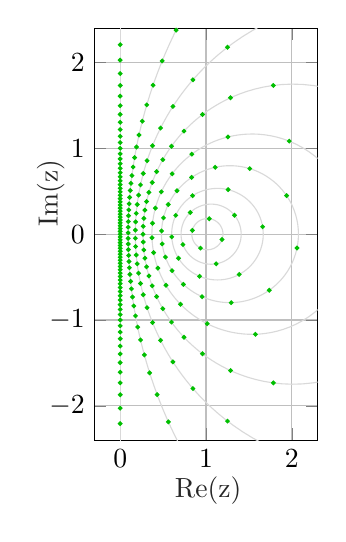
\begin{tikzpicture}

\begin{axis}[%
width=1.1158in,
height=2.0601in,
at={(0,0)},
scale only axis,
unbounded coords=jump,
xmin=-0.3,
xmax=2.3,
ymin=-2.4,
ymax=2.4,
%xmin=-0.1667,
%xmax=2,
%ymin=-2,
%ymax=2,
xlabel style={font=\color{white!15!black},at={(0.51,-0.065)},anchor=north},
xlabel={Re(z)},
xtick={0, 1, 2},
ytick={-2, -1,  0,  1, 2},
ylabel style={font=\color{white!15!black},at={(-0.09,0.6)}},
ylabel={Im(z)},
axis background/.style={fill=white},
xmajorgrids,
ymajorgrids,
legend style={legend cell align=left, align=left, draw=white!15!black}
]
\addplot [color=white!85!black, forget plot]
  table[row sep=crcr]{%
0	0\\
0	-0.0174550649282176\\
0	-0.0349207694917477\\
0	-0.0524077792830412\\
0	-0.0699268119435104\\
0	-0.087488663525924\\
0	-0.105104235265676\\
0	-0.122784560902905\\
0	-0.140540834702391\\
0	-0.158384440324536\\
0	-0.176326980708465\\
0	-0.194380309137718\\
2.22044604925031e-16	-0.212556561670022\\
0	-0.230868191125563\\
0	-0.249328002843181\\
0	-0.267949192431123\\
2.22044604925031e-16	-0.286745385758808\\
0	-0.30573068145866\\
0	-0.324919696232906\\
0	-0.344327613289665\\
2.22044604925031e-16	-0.363970234266202\\
0	-0.383864035035416\\
0	-0.404026225835157\\
0	-0.424474816209605\\
0	-0.445228685308536\\
0	-0.466307658154999\\
0	-0.487732588565861\\
0	-0.509525449494429\\
0	-0.531709431661479\\
0	-0.554309051452769\\
0	-0.577350269189626\\
0	-0.60086061902756\\
0	-0.624869351909328\\
0	-0.649407593197511\\
0	-0.674508516842427\\
0	-0.70020753820971\\
0	-0.726542528005361\\
0	-0.753554050102794\\
0	-0.781285626506717\\
0	-0.809784033195007\\
0	-0.83909963117728\\
0	-0.869286737816226\\
0	-0.90040404429784\\
0	-0.932515086137662\\
0	-0.965688774807074\\
0	-1\\
-1.11022302462516e-16	-1.03553031379057\\
2.22044604925031e-16	-1.07236871002468\\
0	-1.11061251482919\\
-1.11022302462516e-16	-1.15036840722101\\
0	-1.19175359259421\\
0	-1.23489715653505\\
-1.11022302462516e-16	-1.27994163219308\\
0	-1.32704482162041\\
-1.11022302462516e-16	-1.37638192047117\\
0	-1.42814800674211\\
0	-1.48256096851274\\
0	-1.53986496381458\\
0	-1.60033452904105\\
0	-1.66427948235052\\
0	-1.73205080756888\\
0	-1.80404775527142\\
0	-1.88072646534633\\
0	-1.96261050550515\\
-1.11022302462516e-16	-2.0503038415793\\
0	-2.14450692050956\\
0	-2.24603677390422\\
-1.11022302462516e-16	-2.35585236582375\\
0	-2.4750868534163\\
0	-2.6050890646938\\
2.22044604925031e-16	-2.74747741945462\\
-1.11022302462516e-16	-2.90421087767582\\
0	-3.07768353717525\\
2.22044604925031e-16	-3.27085261848414\\
2.22044604925031e-16	-3.48741444384091\\
0	-3.73205080756888\\
2.22044604925031e-16	-4.01078093353584\\
2.22044604925031e-16	-4.33147587428416\\
4.44089209850063e-16	-4.70463010947845\\
2.22044604925031e-16	-5.14455401597031\\
2.22044604925031e-16	-5.67128181961771\\
4.44089209850063e-16	-6.31375151467504\\
1.33226762955019e-15	-7.1153697223842\\
-1.11022302462516e-16	-8.14434642797459\\
-1.99840144432528e-15	-9.51436445422259\\
3.33066907387547e-15	-11.4300523027613\\
2.22044604925031e-15	-14.3006662567119\\
3.5527136788005e-15	-19.0811366877282\\
1.4210854715202e-14	-28.6362532829155\\
-3.71924713249427e-14	-57.2899616307599\\
nan	0\\
-4.87387907810444e-14	57.2899616307595\\
-1.15463194561016e-14	28.6362532829158\\
-3.66373598126302e-15	19.0811366877283\\
5.32907051820075e-15	14.3006662567119\\
1.33226762955019e-15	11.4300523027613\\
4.44089209850063e-16	9.5143644542226\\
-1.88737914186277e-15	8.1443464279746\\
6.66133814775094e-16	7.11536972238421\\
-9.99200722162641e-16	6.31375151467504\\
-1.11022302462516e-16	5.67128181961771\\
-3.33066907387547e-16	5.14455401597031\\
-2.22044604925031e-16	4.70463010947846\\
2.22044604925031e-16	4.33147587428416\\
2.22044604925031e-16	4.01078093353584\\
0	3.73205080756888\\
2.22044604925031e-16	3.48741444384091\\
-2.22044604925031e-16	3.27085261848414\\
2.22044604925031e-16	3.07768353717525\\
2.22044604925031e-16	2.90421087767583\\
0	2.74747741945462\\
0	2.6050890646938\\
0	2.4750868534163\\
2.22044604925031e-16	2.35585236582375\\
0	2.24603677390422\\
0	2.14450692050956\\
0	2.0503038415793\\
0	1.96261050550515\\
0	1.88072646534633\\
0	1.80404775527142\\
-2.22044604925031e-16	1.73205080756888\\
-2.22044604925031e-16	1.66427948235052\\
0	1.60033452904105\\
0	1.53986496381458\\
0	1.48256096851274\\
0	1.42814800674212\\
0	1.37638192047117\\
0	1.32704482162041\\
-1.11022302462516e-16	1.27994163219308\\
-1.11022302462516e-16	1.23489715653505\\
0	1.19175359259421\\
2.22044604925031e-16	1.15036840722101\\
0	1.11061251482919\\
0	1.07236871002468\\
2.22044604925031e-16	1.03553031379057\\
0	1\\
0	0.965688774807074\\
0	0.932515086137662\\
0	0.90040404429784\\
0	0.869286737816227\\
0	0.83909963117728\\
0	0.809784033195008\\
0	0.781285626506718\\
0	0.753554050102794\\
0	0.726542528005361\\
0	0.70020753820971\\
0	0.674508516842427\\
0	0.64940759319751\\
0	0.624869351909328\\
0	0.600860619027561\\
0	0.577350269189626\\
0	0.554309051452769\\
0	0.531709431661479\\
0	0.509525449494429\\
0	0.487732588565861\\
0	0.466307658154999\\
0	0.445228685308536\\
0	0.424474816209605\\
0	0.404026225835157\\
0	0.383864035035416\\
0	0.363970234266203\\
0	0.344327613289666\\
0	0.324919696232906\\
0	0.305730681458661\\
0	0.286745385758808\\
0	0.267949192431123\\
0	0.249328002843181\\
0	0.230868191125563\\
0	0.212556561670022\\
0	0.194380309137719\\
0	0.176326980708465\\
0	0.158384440324536\\
0	0.140540834702392\\
0	0.122784560902905\\
0	0.105104235265677\\
0	0.0874886635259245\\
2.22044604925031e-16	0.0699268119435106\\
0	0.0524077792830412\\
0	0.0349207694917475\\
0	0.0174550649282175\\
0	1.22464679914735e-16\\
};
\addplot [color=white!85!black, forget plot]
  table[row sep=crcr]{%
0.0928961748633879	0\\
0.0929242340793204	-0.0173043874682864\\
0.0930084792643229	-0.0346190494354207\\
0.0931491133740723	-0.0519542844799809\\
0.093346475817897	-0.0693204394581452\\
0.0936010441941062	-0.0867279339388205\\
0.0939134367406476	-0.104187284997116\\
0.0942844155226323	-0.121709132490233\\
0.0947148903849062	-0.139304264943875\\
0.0952059237048746	-0.156983646182423\\
0.0957587359882799	-0.174758442842423\\
0.0963747123587413	-0.1926400529165\\
0.0970554100006449	-0.21064013548368\\
0.0978025666246207	-0.228770641792508\\
0.0986181100354775	-0.247043847875266\\
0.0995041688942513	-0.265472388885338\\
0.100463084779183	-0.284069295365409\\
0.101497425665167	-0.302848031672029\\
0.102610000957802	-0.32182253680226\\
0.103803878236859	-0.341007267891088\\
0.105082401885219	-0.360417246674213\\
0.106449213803392	-0.380068109240183\\
0.107908276437208	-0.399976159429091\\
0.109463898377632	-0.420158426272597\\
0.111120762827617	-0.440632725912625\\
0.112883959272193	-0.461417728484205\\
0.114759018735544	-0.482533030502606\\
0.116751953063696	-0.503999233356777\\
0.118869298734931	-0.525838028581534\\
0.121118165773682	-0.54807229066084\\
0.123506292429235	-0.570726178205633\\
0.126042106380326	-0.593825244453381\\
0.128734793343232	-0.617396558155023\\
0.131594374097383	-0.641468836050322\\
0.134631791102734	-0.666072588287666\\
0.137859006071691	-0.69124027832203\\
0.141289110080938	-0.717006499028841\\
0.144936448071905	-0.743408167006151\\
0.148816759901222	-0.770484737307809\\
0.152947340474577	-0.798278441162159\\
0.157347221941592	-0.826834549591131\\
0.162037381461288	-0.856201666261631\\
0.167040978686694	-0.886432053384504\\
0.172383627887389	-0.917581995037453\\
0.178093710560155	-0.949712202940524\\
0.184202735508319	-0.982888270471905\\
0.190745754747132	-1.01718118159632\\
0.197761845275717	-1.05266788241005\\
0.205294668821916	-1.08943192421082\\
0.213393124211853	-1.12756418840683\\
0.222112110165757	-1.16716370522138\\
0.231513420235663	-1.2083385800655\\
0.2416667964863	-1.25120704368485\\
0.252651174647097	-1.29589864478511\\
0.264556161182823	-1.34255560685138\\
0.27748379250524	-1.39133437434931\\
0.291550638989107	-1.44240737746862\\
0.306890332374032	-1.49596504906346\\
0.323656615612751	-1.55221813244105\\
0.342027040722491	-1.61140032406189\\
0.362207474676912	-1.67377130082916\\
0.384437618517587	-1.73962018703981\\
0.408997804325234	-1.80926952046835\\
0.436217413506038	-1.88307977909351\\
0.46648536498124	-1.96145452731893\\
0.500263263003183	-2.04484622923645\\
0.53810198498856	-2.13376274992215\\
0.580662748934347	-2.2287745129058\\
0.628744054333606	-2.33052218439028\\
0.683316377524968	-2.43972458169992\\
0.745567174603139	-2.55718620302048\\
0.816959675270921	-2.68380326027553\\
0.899310238575398	-2.82056621819545\\
0.994890816534536	-2.96855534553194\\
1.10656549238336	-3.12892322974095\\
1.23797328591861	-3.30285383256975\\
1.39377351865458	-3.49148014488623\\
1.57997473174728	-3.69572952809174\\
1.8043721801811	-3.91604342811807\\
2.07711842748108	-4.15187961645313\\
2.41143631003606	-4.40083977933\\
2.82442833394503	-4.65715830475088\\
3.33778282556612	-4.90912654988277\\
3.97779826577577	-5.13482926595128\\
4.77330390774541	-5.29548903622297\\
5.74842943708677	-5.32632314910675\\
6.90489311590568	-5.12767323042671\\
8.18820960335285	-4.56700612281641\\
9.44339042885261	-3.51496124525747\\
10.4007768874728	-1.93683676831165\\
10.7647058823529	-7.03430341378756e-15\\
10.4007768874728	1.93683676831166\\
9.44339042885263	3.51496124525745\\
8.18820960335288	4.56700612281639\\
6.90489311590569	5.12767323042671\\
5.74842943708676	5.32632314910675\\
4.77330390774541	5.29548903622297\\
3.97779826577578	5.13482926595129\\
3.33778282556613	4.90912654988277\\
2.82442833394502	4.65715830475088\\
2.41143631003606	4.40083977933\\
2.07711842748108	4.15187961645313\\
1.80437218018111	3.91604342811807\\
1.57997473174728	3.69572952809174\\
1.39377351865458	3.49148014488624\\
1.23797328591861	3.30285383256974\\
1.10656549238336	3.12892322974095\\
0.994890816534536	2.96855534553194\\
0.899310238575398	2.82056621819546\\
0.816959675270923	2.68380326027553\\
0.745567174603139	2.55718620302048\\
0.683316377524968	2.43972458169992\\
0.628744054333606	2.33052218439028\\
0.580662748934348	2.2287745129058\\
0.53810198498856	2.13376274992215\\
0.500263263003183	2.04484622923645\\
0.46648536498124	1.96145452731893\\
0.436217413506038	1.88307977909351\\
0.408997804325235	1.80926952046835\\
0.384437618517587	1.73962018703981\\
0.362207474676913	1.67377130082916\\
0.342027040722491	1.61140032406189\\
0.323656615612752	1.55221813244105\\
0.306890332374032	1.49596504906346\\
0.291550638989108	1.44240737746862\\
0.27748379250524	1.39133437434931\\
0.264556161182823	1.34255560685138\\
0.252651174647097	1.29589864478511\\
0.2416667964863	1.25120704368485\\
0.231513420235663	1.2083385800655\\
0.222112110165757	1.16716370522138\\
0.213393124211853	1.12756418840683\\
0.205294668821916	1.08943192421082\\
0.197761845275717	1.05266788241005\\
0.190745754747132	1.01718118159632\\
0.184202735508319	0.982888270471905\\
0.178093710560155	0.949712202940524\\
0.172383627887389	0.917581995037453\\
0.167040978686694	0.886432053384505\\
0.162037381461288	0.856201666261631\\
0.157347221941592	0.826834549591131\\
0.152947340474577	0.79827844116216\\
0.148816759901223	0.77048473730781\\
0.144936448071905	0.743408167006151\\
0.141289110080938	0.717006499028841\\
0.137859006071691	0.69124027832203\\
0.134631791102734	0.666072588287666\\
0.131594374097383	0.641468836050322\\
0.128734793343232	0.617396558155023\\
0.126042106380326	0.593825244453382\\
0.123506292429235	0.570726178205633\\
0.121118165773682	0.54807229066084\\
0.118869298734931	0.525838028581534\\
0.116751953063696	0.503999233356777\\
0.114759018735545	0.482533030502606\\
0.112883959272193	0.461417728484205\\
0.111120762827617	0.440632725912625\\
0.109463898377632	0.420158426272598\\
0.107908276437208	0.399976159429091\\
0.106449213803392	0.380068109240183\\
0.105082401885219	0.360417246674213\\
0.103803878236859	0.341007267891088\\
0.102610000957802	0.32182253680226\\
0.101497425665167	0.30284803167203\\
0.100463084779183	0.28406929536541\\
0.0995041688942513	0.265472388885338\\
0.0986181100354775	0.247043847875266\\
0.0978025666246207	0.228770641792508\\
0.0970554100006449	0.21064013548368\\
0.0963747123587415	0.1926400529165\\
0.0957587359882799	0.174758442842423\\
0.0952059237048746	0.156983646182423\\
0.0947148903849064	0.139304264943875\\
0.0942844155226321	0.121709132490233\\
0.0939134367406476	0.104187284997116\\
0.0936010441941062	0.086727933938821\\
0.093346475817897	0.0693204394581455\\
0.0931491133740723	0.0519542844799809\\
0.0930084792643229	0.0346190494354204\\
0.0929242340793204	0.0173043874682863\\
0.0928961748633879	1.2140784655168e-16\\
};
\addplot [color=white!85!black, forget plot]
  table[row sep=crcr]{%
0.176470588235294	0\\
0.176522680272067	-0.0169113211319614\\
0.176679077471975	-0.0338319866673218\\
0.176940143691687	-0.0507713604600582\\
0.17730648732347	-0.0677388453443164\\
0.177778964258808	-0.0847439028225076\\
0.178358682071455	-0.101796072992362\\
0.17904700545442	-0.11890499479484\\
0.179845562955953	-0.136080426666741\\
0.180756255070742	-0.153332267684324\\
0.181781263754378	-0.170670579287198\\
0.182923063441847	-0.188105607675322\\
0.184184433664552	-0.205647806975985\\
0.185568473375314	-0.223307863282371\\
0.187078617107208	-0.241096719670592\\
0.188718653110133	-0.259025602308026\\
0.190492743629048	-0.277106047772426\\
0.192405447510008	-0.295349931708615\\
0.194461745345025	-0.313769498957655\\
0.196667067394564	-0.332377395302257\\
0.199027324557801	-0.351186700981847\\
0.201548942696	-0.370210966141226\\
0.204238900654229	-0.389464248388089\\
0.207104772371764	-0.408961152646904\\
0.210154773522759	-0.42871687350968\\
0.213397813187101	-0.448747240298056\\
0.21684355111781	-0.469068765065773\\
0.220502461247311	-0.4896986937859\\
0.224385902161824	-0.510655060983012\\
0.228506195372787	-0.531956748086621\\
0.232876712328767	-0.553623545798271\\
0.237511971243092	-0.57567622078034\\
0.242427744964446	-0.598136586989191\\
0.247641181293201	-0.621027581988062\\
0.253170937349436	-0.644373348584925\\
0.259037329834106	-0.668199322146024\\
0.265262503298337	-0.692532323935113\\
0.271870618854103	-0.717400660819007\\
0.278888066130376	-0.742834231658732\\
0.286343701711988	-0.768864640668127\\
0.294269117804919	-0.79552531796252\\
0.302698945465215	-0.822851647432014\\
0.311671197425291	-0.850881101947331\\
0.321227656370161	-0.87965338572887\\
0.331414315480287	-0.909210583465365\\
0.342281879194631	-0.939597315436242\\
0.35388633349005	-0.970860897443779\\
0.366289596560616	-1.0030515037613\\
0.379560262659437	-1.03622233050424\\
0.393774454091766	-1.07042975576962\\
0.409016798987261	-1.10573349148401\\
0.42538155560874	-1.14219672004146\\
0.442973907665055	-1.17988620635853\\
0.461911459491316	-1.21887237273246\\
0.482325965159465	-1.25922931960894\\
0.504365331717945	-1.30103476971338\\
0.52819594397216	-1.34436990552571\\
0.554005366649542	-1.38931906019066\\
0.582005489571341	-1.43596920885532\\
0.612436192661469	-1.48440919005134\\
0.645569620253164	-1.53472856366863\\
0.68171516802733	-1.58701598139833\\
0.721225300550089	-1.64135690471893\\
0.764502331775035	-1.69783045118312\\
0.8120063131902	-1.75650507746391\\
0.864264181287679	-1.81743271146486\\
0.921880312257394	-1.8806408181745\\
0.985548608266636	-1.94612171516153\\
1.05606618184676	-2.01381823170575\\
1.13434858960967	-2.08360451651563\\
1.22144635737572	-2.15526042781376\\
1.3185621794694	-2.22843747335106\\
1.42706757965902	-2.30261370252471\\
1.54851686226186	-2.37703430665543\\
1.68465467496922	-2.45063402389295\\
1.83741119624329	-2.5219369360202\\
2.00887552721665	-2.58892922840514\\
2.20123296065471	-2.64890161615092\\
2.41664517759302	-2.69826158010845\\
2.65704429562471	-2.73232320979376\\
2.92380343125746	-2.74509712953071\\
3.21724184883905	-2.72912817417207\\
3.53592997176006	-2.67546694681967\\
3.87579275196896	-2.57391133590372\\
4.22908860276105	-2.41370146436359\\
4.58348085995945	-2.18485948663627\\
4.9216063495083	-1.88026922414147\\
5.22169972829057	-1.49831911282485\\
5.45978161072782	-1.04548462276147\\
5.61347325851817	-0.537784996206515\\
5.66666666666667	-1.90500613200699e-15\\
5.61347325851817	0.537784996206518\\
5.45978161072782	1.04548462276146\\
5.22169972829058	1.49831911282484\\
4.92160634950831	1.88026922414146\\
4.58348085995945	2.18485948663627\\
4.22908860276106	2.41370146436359\\
3.87579275196897	2.57391133590372\\
3.53592997176007	2.67546694681966\\
3.21724184883905	2.72912817417208\\
2.92380343125746	2.74509712953071\\
2.65704429562471	2.73232320979376\\
2.41664517759302	2.69826158010845\\
2.20123296065472	2.64890161615093\\
2.00887552721665	2.58892922840514\\
1.83741119624329	2.5219369360202\\
1.68465467496922	2.45063402389295\\
1.54851686226186	2.37703430665543\\
1.42706757965902	2.30261370252471\\
1.3185621794694	2.22843747335107\\
1.22144635737572	2.15526042781376\\
1.13434858960967	2.08360451651563\\
1.05606618184675	2.01381823170575\\
0.985548608266636	1.94612171516153\\
0.921880312257395	1.8806408181745\\
0.864264181287679	1.81743271146486\\
0.8120063131902	1.75650507746391\\
0.764502331775035	1.69783045118312\\
0.72122530055009	1.64135690471894\\
0.68171516802733	1.58701598139833\\
0.645569620253165	1.53472856366863\\
0.612436192661469	1.48440919005134\\
0.582005489571341	1.43596920885532\\
0.554005366649542	1.38931906019066\\
0.52819594397216	1.34436990552571\\
0.504365331717945	1.30103476971338\\
0.482325965159465	1.25922931960894\\
0.461911459491315	1.21887237273246\\
0.442973907665055	1.17988620635853\\
0.42538155560874	1.14219672004146\\
0.409016798987261	1.10573349148401\\
0.393774454091766	1.07042975576962\\
0.379560262659437	1.03622233050424\\
0.366289596560616	1.0030515037613\\
0.35388633349005	0.97086089744378\\
0.342281879194631	0.939597315436242\\
0.331414315480287	0.909210583465365\\
0.321227656370161	0.87965338572887\\
0.311671197425291	0.850881101947332\\
0.302698945465215	0.822851647432015\\
0.294269117804919	0.795525317962521\\
0.286343701711988	0.768864640668127\\
0.278888066130376	0.742834231658732\\
0.271870618854103	0.717400660819007\\
0.265262503298337	0.692532323935113\\
0.259037329834106	0.668199322146024\\
0.253170937349436	0.644373348584925\\
0.247641181293201	0.621027581988062\\
0.242427744964446	0.598136586989191\\
0.237511971243092	0.575676220780341\\
0.232876712328767	0.553623545798271\\
0.228506195372787	0.531956748086621\\
0.224385902161824	0.510655060983012\\
0.220502461247311	0.4896986937859\\
0.21684355111781	0.469068765065772\\
0.213397813187101	0.448747240298056\\
0.210154773522759	0.42871687350968\\
0.207104772371764	0.408961152646905\\
0.204238900654229	0.389464248388089\\
0.201548942696	0.370210966141226\\
0.199027324557801	0.351186700981848\\
0.196667067394564	0.332377395302257\\
0.194461745345025	0.313769498957655\\
0.192405447510008	0.295349931708615\\
0.190492743629048	0.277106047772426\\
0.188718653110133	0.259025602308026\\
0.187078617107208	0.241096719670592\\
0.185568473375314	0.22330786328237\\
0.184184433664552	0.205647806975985\\
0.182923063441847	0.188105607675323\\
0.181781263754378	0.170670579287198\\
0.180756255070742	0.153332267684324\\
0.179845562955953	0.136080426666742\\
0.17904700545442	0.11890499479484\\
0.178358682071455	0.101796072992362\\
0.177778964258808	0.0847439028225081\\
0.17730648732347	0.0677388453443166\\
0.176940143691687	0.0507713604600582\\
0.176679077471975	0.0338319866673216\\
0.176522680272067	0.0169113211319613\\
0.176470588235294	1.18650900955453e-16\\
};
\addplot [color=white!85!black, forget plot]
  table[row sep=crcr]{%
0.265822784810126	0\\
0.265898050942813	-0.0162213102115928\\
0.266124013410003	-0.0324504104803718\\
0.266501165145765	-0.0486951030922275\\
0.267030330134381	-0.0649632148137771\\
0.267712667069969	-0.0812626091908714\\
0.268549674516907	-0.0976011989164377\\
0.269543197608459	-0.11398695829003\\
0.270695436332347	-0.130427935790774\\
0.272008955463872	-0.146932266784504\\
0.273486696219659	-0.163508186384728\\
0.275131989718365	-0.180164042485595\\
0.276948572348816	-0.196908308983242\\
0.278940603161286	-0.213749599199617\\
0.281112683414095	-0.230696679520143\\
0.283469878425554	-0.247758483253196\\
0.286017741900838	-0.264944124715269\\
0.288762342924724	-0.282262913540667\\
0.291710295834605	-0.299724369208572\\
0.294868793214104	-0.317338235772939\\
0.298245642276169	-0.335114496771889\\
0.301849304936205	-0.353063390282575\\
0.305688941910884	-0.371195424074704\\
0.309774461217269	-0.389521390800437\\
0.314116571490255	-0.408052383139892\\
0.318726840584625	-0.42679980879921\\
0.323617759981813	-0.445775405231455\\
0.328802815581534	-0.464991253918625\\
0.334296565525388	-0.484459794014648\\
0.34011472577434	-0.504193835103263\\
0.34627426424546	-0.524206568769541\\
0.352793504406507	-0.544511578617706\\
0.359692239330959	-0.565122848288713\\
0.366991857332091	-0.586054766936049\\
0.374715480424017	-0.607322131504291\\
0.382888117001453	-0.62894014501829\\
0.391536830289885	-0.650924409926799\\
0.400690924295007	-0.673290915347343\\
0.410382149176274	-0.696056016822496\\
0.420644928185159	-0.719236406913174\\
0.431516608545333	-0.742849074612439\\
0.443037738909736	-0.766911251151508\\
0.455252376308314	-0.791440339273936\\
0.468208425798595	-0.816453822456737\\
0.481958016346465	-0.841969149837512\\
0.49655791679138	-0.868003591739\\
0.51206999608052	-0.894574059636089\\
0.528561732277561	-0.921696883148368\\
0.546106775144948	-0.949387535119208\\
0.564785567337015	-0.977660294007125\\
0.584686029386328	-1.00652783060336\\
0.605904313663554	-1.03600070342639\\
0.628545632266937	-1.06608674394114\\
0.652725163247935	-1.09679030890624\\
0.67856903856368	-1.12811137254862\\
0.70621541547276	-1.16004442577126\\
0.735815630499326	-1.19257714307226\\
0.767535431233344	-1.22568877014505\\
0.801556275647149	-1.25934817609622\\
0.838076680673205	-1.29351150374422\\
0.877313590692755	-1.32811933948962\\
0.919503721269278	-1.36309331083205\\
0.964904812554868	-1.39833200499505\\
1.01379669855786	-1.4337060868753\\
1.06648206070523	-1.46905247972074\\
1.12328668420254	-1.50416745939867\\
1.18455897045367	-1.53879850582272\\
1.25066837475506	-1.57263475772146\\
1.32200233206178	-1.60529593648329\\
1.39896110183541	-1.63631965159517\\
1.48194980454385	-1.66514708882503\\
1.57136673971757	-1.69110723280973\\
1.66758687790764	-1.71340001439218\\
1.77093922752017	-1.7310791324117\\
1.8816766320022	-1.74303581641394\\
1.99993652033888	-1.74798550602253\\
2.12569131862878	-1.74446034571155\\
2.25868778196976	-1.73081151557542\\
2.39837561762634	-1.7052266533392\\
2.54382765981905	-1.66576876447122\\
2.69365670758171	-1.61044368551659\\
2.84593798907048	-1.53730276692232\\
2.99815078733475	-1.44458519020414\\
3.14715723780444	-1.33089940306667\\
3.28923916983732	-1.19543502361914\\
3.42021295283882	-1.03818557253197\\
3.53563532042957	-0.860150368344511\\
3.63109872482125	-0.663474497931426\\
3.70259395673031	-0.451483848445247\\
3.74689507708525	-0.228582147030333\\
3.76190476190476	-8.05323291956309e-16\\
3.74689507708525	0.228582147030334\\
3.70259395673031	0.451483848445243\\
3.63109872482125	0.663474497931422\\
3.53563532042957	0.86015036834451\\
3.42021295283882	1.03818557253198\\
3.28923916983732	1.19543502361914\\
3.14715723780444	1.33089940306667\\
2.99815078733476	1.44458519020413\\
2.84593798907048	1.53730276692232\\
2.69365670758171	1.61044368551658\\
2.54382765981905	1.66576876447122\\
2.39837561762634	1.7052266533392\\
2.25868778196976	1.73081151557542\\
2.12569131862879	1.74446034571155\\
1.99993652033888	1.74798550602253\\
1.88167663200221	1.74303581641394\\
1.77093922752017	1.7310791324117\\
1.66758687790764	1.71340001439218\\
1.57136673971757	1.69110723280973\\
1.48194980454386	1.66514708882503\\
1.39896110183541	1.63631965159517\\
1.32200233206177	1.60529593648329\\
1.25066837475507	1.57263475772146\\
1.18455897045368	1.53879850582272\\
1.12328668420254	1.50416745939867\\
1.06648206070523	1.46905247972074\\
1.01379669855786	1.4337060868753\\
0.964904812554869	1.39833200499505\\
0.919503721269278	1.36309331083205\\
0.877313590692756	1.32811933948962\\
0.838076680673205	1.29351150374422\\
0.80155627564715	1.25934817609622\\
0.767535431233344	1.22568877014505\\
0.735815630499326	1.19257714307226\\
0.70621541547276	1.16004442577126\\
0.67856903856368	1.12811137254862\\
0.652725163247935	1.09679030890624\\
0.628545632266937	1.06608674394114\\
0.605904313663554	1.03600070342639\\
0.584686029386328	1.00652783060336\\
0.564785567337015	0.977660294007125\\
0.546106775144948	0.949387535119208\\
0.528561732277561	0.921696883148368\\
0.512069996080521	0.89457405963609\\
0.49655791679138	0.868003591739001\\
0.481958016346465	0.841969149837512\\
0.468208425798595	0.816453822456737\\
0.455252376308315	0.791440339273937\\
0.443037738909736	0.766911251151508\\
0.431516608545333	0.742849074612439\\
0.420644928185159	0.719236406913174\\
0.410382149176274	0.696056016822496\\
0.400690924295007	0.673290915347343\\
0.391536830289885	0.650924409926799\\
0.382888117001454	0.628940145018291\\
0.374715480424017	0.607322131504291\\
0.366991857332091	0.586054766936049\\
0.359692239330959	0.565122848288713\\
0.352793504406508	0.544511578617706\\
0.34627426424546	0.524206568769541\\
0.340114725774341	0.504193835103263\\
0.334296565525388	0.484459794014648\\
0.328802815581534	0.464991253918625\\
0.323617759981813	0.445775405231455\\
0.318726840584625	0.42679980879921\\
0.314116571490256	0.408052383139893\\
0.309774461217269	0.389521390800438\\
0.305688941910884	0.371195424074705\\
0.301849304936205	0.353063390282575\\
0.298245642276169	0.335114496771889\\
0.294868793214104	0.31733823577294\\
0.291710295834606	0.299724369208572\\
0.288762342924724	0.282262913540667\\
0.286017741900838	0.264944124715269\\
0.283469878425554	0.247758483253197\\
0.281112683414095	0.230696679520143\\
0.278940603161286	0.213749599199617\\
0.276948572348816	0.196908308983242\\
0.275131989718365	0.180164042485595\\
0.273486696219659	0.163508186384727\\
0.272008955463872	0.146932266784504\\
0.270695436332347	0.130427935790774\\
0.269543197608459	0.11398695829003\\
0.268549674516907	0.097601198916438\\
0.267712667069969	0.0812626091908718\\
0.267030330134381	0.0649632148137773\\
0.266501165145765	0.0486951030922275\\
0.266124013410003	0.0324504104803715\\
0.265898050942813	0.0162213102115927\\
0.265822784810126	1.13811110960658e-16\\
};
\addplot [color=white!85!black, forget plot]
  table[row sep=crcr]{%
0.36986301369863	0\\
0.36996028346031	-0.0150666076576168\\
0.370252281231189	-0.0301386276657198\\
0.370739573165269	-0.045221474920134\\
0.371423105177891	-0.0603205693690484\\
0.372304206446904	-0.0754413384427429\\
0.373384594340659	-0.0905892193656722\\
0.374666380799405	-0.105769661308501\\
0.376152080204487	-0.120988127334879\\
0.377844618777794	-0.136250096094146\\
0.379747345562214	-0.151561063206738\\
0.381864045042391	-0.166926542283666\\
0.384198951473995	-0.18235206551511\\
0.386756764998974	-0.197843183755646\\
0.389542669633901	-0.213405466024899\\
0.392562353228645	-0.229044498332289\\
0.395822029503159	-0.24476588172283\\
0.399328462281248	-0.260575229427492\\
0.403088992051746	-0.276478162986172\\
0.407111564999665	-0.292480307193613\\
0.411404764662461	-0.308587283698318\\
0.41597784637974	-0.324804703061305\\
0.420840774718247	-0.341138155055049\\
0.426004264068019	-0.357593196952631\\
0.431479822619771	-0.374175339522531\\
0.437279799948024	-0.390890030404989\\
0.443417438438768	-0.407742634500731\\
0.449906928814442	-0.424738410951407\\
0.456763470022259	-0.4418824862323\\
0.464003333763978	-0.45917982281085\\
0.471643933955492	-0.476635182748076\\
0.479703901412286	-0.494253085532792\\
0.488203164060909	-0.512037759339133\\
0.497163032975849	-0.529993084784719\\
0.506606294534026	-0.548122530137934\\
0.51655730896351	-0.566429076776197\\
0.527042115536528	-0.584915133530642\\
0.538088544616377	-0.603582438363631\\
0.549726336709481	-0.622431945611521\\
0.561987268592996	-0.641463696783117\\
0.574905286479098	-0.660676672631322\\
0.588516646032246	-0.680068623908586\\
0.602860058866567	-0.699635877872834\\
0.617976844906173	-0.719373117226887\\
0.633911089678764	-0.739273127748586\\
0.650709805216243	-0.759326510399472\\
0.66842309273618	-0.779521353186721\\
0.687104304651664	-0.799842857497885\\
0.70681020267669	-0.820272913035417\\
0.727601107827008	-0.840789614856813\\
0.749541036923469	-0.861366715390662\\
0.772697818741185	-0.881973003671259\\
0.797143181161087	-0.902571603447238\\
0.822952798511357	-0.923119181319477\\
0.850206285668862	-0.943565055715414\\
0.878987122353232	-0.963850197399643\\
0.909382487314417	-0.983906112474146\\
0.941482977714772	-1.00365359959415\\
0.975382183874672	-1.02300137462482\\
1.01117608364116	-1.04184455845622\\
1.04896221394359	-1.06006302751688\\
1.08883856966921	-1.07751963209955\\
1.13090217196943	-1.09405829544777\\
1.17524723977324	-1.1095020172543\\
1.22196289011556	-1.12365081948992\\
1.2711302856283	-1.13627969107424\\
1.32281914229396	-1.14713661160216\\
1.37708350888763	-1.15594076385876\\
1.4339567335581	-1.16238108068848\\
1.49344554550216	-1.16611531399256\\
1.55552320414814	-1.16676986152945\\
1.62012170881876	-1.16394063894192\\
1.68712312307348	-1.15719533650517\\
1.75635015441019	-1.14607744668627\\
1.82755624549549	-1.13011248107705\\
1.90041557927088	-1.10881680170548\\
1.97451357498608	-1.08170945698556\\
2.04933864722677	-1.04832731901123\\
2.12427619866686	-1.00824364841534\\
2.19860599245205	-0.961089950543595\\
2.27150416346192	-0.90658062555547\\
2.34205113142678	-0.844539463725866\\
2.40924652139591	-0.774926526402034\\
2.47203183329182	-0.697863441051832\\
2.52932100842074	-0.61365471192682\\
2.58003823113275	-0.522802412703495\\
2.62316134493291	-0.426011693045989\\
2.6577682781299	-0.324184981136075\\
2.68308303501967	-0.218403625548967\\
2.6985173020487	-0.109896935603413\\
2.7037037037037	-3.86376905080784e-16\\
2.6985173020487	0.109896935603413\\
2.68308303501967	0.218403625548965\\
2.6577682781299	0.324184981136073\\
2.62316134493291	0.426011693045989\\
2.58003823113275	0.522802412703496\\
2.52932100842074	0.613654711926819\\
2.47203183329182	0.697863441051831\\
2.40924652139591	0.774926526402033\\
2.34205113142678	0.844539463725866\\
2.27150416346192	0.906580625555469\\
2.19860599245205	0.961089950543594\\
2.12427619866687	1.00824364841534\\
2.04933864722677	1.04832731901123\\
1.97451357498608	1.08170945698556\\
1.90041557927088	1.10881680170548\\
1.82755624549549	1.13011248107705\\
1.75635015441019	1.14607744668627\\
1.68712312307349	1.15719533650517\\
1.62012170881876	1.16394063894192\\
1.55552320414814	1.16676986152946\\
1.49344554550216	1.16611531399256\\
1.4339567335581	1.16238108068848\\
1.37708350888763	1.15594076385876\\
1.32281914229396	1.14713661160216\\
1.2711302856283	1.13627969107424\\
1.22196289011556	1.12365081948992\\
1.17524723977324	1.1095020172543\\
1.13090217196943	1.09405829544777\\
1.08883856966921	1.07751963209955\\
1.04896221394359	1.06006302751688\\
1.01117608364116	1.04184455845622\\
0.975382183874673	1.02300137462482\\
0.941482977714772	1.00365359959415\\
0.909382487314417	0.983906112474146\\
0.878987122353232	0.963850197399644\\
0.850206285668862	0.943565055715414\\
0.822952798511357	0.923119181319477\\
0.797143181161087	0.902571603447238\\
0.772697818741186	0.88197300367126\\
0.749541036923469	0.861366715390662\\
0.727601107827007	0.840789614856813\\
0.70681020267669	0.820272913035417\\
0.687104304651665	0.799842857497885\\
0.668423092736181	0.779521353186722\\
0.650709805216243	0.759326510399472\\
0.633911089678764	0.739273127748586\\
0.617976844906173	0.719373117226888\\
0.602860058866567	0.699635877872834\\
0.588516646032246	0.680068623908586\\
0.574905286479098	0.660676672631322\\
0.561987268592996	0.641463696783117\\
0.549726336709481	0.622431945611521\\
0.538088544616377	0.603582438363631\\
0.527042115536528	0.584915133530642\\
0.51655730896351	0.566429076776197\\
0.506606294534026	0.548122530137934\\
0.497163032975849	0.529993084784719\\
0.488203164060909	0.512037759339133\\
0.479703901412287	0.494253085532792\\
0.471643933955492	0.476635182748076\\
0.464003333763978	0.45917982281085\\
0.456763470022259	0.441882486232301\\
0.449906928814442	0.424738410951407\\
0.443417438438768	0.40774263450073\\
0.437279799948024	0.390890030404989\\
0.431479822619771	0.374175339522532\\
0.426004264068019	0.357593196952632\\
0.420840774718247	0.34113815505505\\
0.41597784637974	0.324804703061305\\
0.411404764662462	0.308587283698318\\
0.407111564999665	0.292480307193614\\
0.403088992051746	0.276478162986172\\
0.399328462281247	0.260575229427492\\
0.395822029503159	0.244765881722831\\
0.392562353228645	0.229044498332289\\
0.389542669633901	0.213405466024899\\
0.386756764998974	0.197843183755646\\
0.384198951473995	0.18235206551511\\
0.381864045042391	0.166926542283666\\
0.379747345562214	0.151561063206738\\
0.377844618777794	0.136250096094146\\
0.376152080204487	0.120988127334879\\
0.374666380799405	0.105769661308501\\
0.373384594340658	0.0905892193656724\\
0.372304206446904	0.0754413384427433\\
0.371423105177891	0.0603205693690486\\
0.370739573165269	0.045221474920134\\
0.370252281231189	0.0301386276657196\\
0.36996028346031	0.0150666076576167\\
0.36986301369863	1.05711677164155e-16\\
};
\addplot [color=white!85!black, forget plot]
  table[row sep=crcr]{%
0.481481481481481	0\\
0.481594162911531	-0.0134076076698943\\
0.481932386364852	-0.0268177010816324\\
0.482496689791934	-0.040232759271768\\
0.483287971314349	-0.0536552477916375\\
0.484307491533934	-0.0670876117774552\\
0.485556876771667	-0.0805322687936767\\
0.487038123242121	-0.093991601370743\\
0.488753602170918	-0.107467949155439\\
0.490706065863888	-0.120963600588455\\
0.492898654737874	-0.134480784019298\\
0.495334905323979	-0.148021658163403\\
0.498018759254725	-0.161588301800148\\
0.500954573246841	-0.175182702603322\\
0.504147130091255	-0.188806744987549\\
0.507601650661167	-0.20246219684491\\
0.511323806947811	-0.216150695035776\\
0.515319736131428	-0.229873729486243\\
0.519596055692128	-0.243632625731761\\
0.524159879561291	-0.257428525732258\\
0.529018835309021	-0.27126236676833\\
0.534181082356516	-0.285134858210658\\
0.53965533119387	-0.299046455935784\\
0.54545086357347	-0.312997334140444\\
0.55157755363645	-0.326987354283858\\
0.55804588991418	-0.341016030862564\\
0.564866998128088	-0.355082493695427\\
0.572052664688631	-0.369185446367411\\
0.579615360767372	-0.383323120449387\\
0.587568266784194	-0.39749322507782\\
0.595925297113752	-0.411692891442517\\
0.604701124770527	-0.425918611693055\\
0.613911205779188	-0.440166171735013\\
0.6235718028751	-0.454430577346312\\
0.633700008107486	-0.46870597300202\\
0.644313763833332	-0.482985552753828\\
0.655431881491931	-0.49726146246877\\
0.667074057436035	-0.511524692691958\\
0.6792608849639	-0.525764961361648\\
0.692013861544633	-0.539970585573895\\
0.705355390054875	-0.554128341570933\\
0.719308772645196	-0.568223312115509\\
0.733898195627031	-0.58223872041669\\
0.749148703512763	-0.596155749796195\\
0.765086160050017	-0.609953348334217\\
0.78173719376392	-0.623608017817372\\
0.799129125156153	-0.63709358643806\\
0.817289872305732	-0.650380964874699\\
0.83624783117367	-0.663437885629073\\
0.856031726433461	-0.676228625825348\\
0.876670428135553	-0.688713714102675\\
0.898192728973515	-0.700849622779937\\
0.920627076363435	-0.71258844715964\\
0.94400125299236	-0.723877574693485\\
0.968341998959287	-0.734659347782055\\
0.993674568154574	-0.744870725253828\\
1.02002221114227	-0.75444294909338\\
1.04740557657865	-0.763301224792098\\
1.07584202318755	-0.771364425800108\\
1.10534483460426	-0.778544834980075\\
1.13592233009709	-0.784747938704346\\
1.16757686540324	-0.789872292279264\\
1.20030371981325	-0.79380947868027\\
1.23408986836534	-0.796444186057494\\
1.26891264173706	-0.797654432995354\\
1.30473828131947	-0.797311973892388\\
1.3415204031896	-0.795282919808421\\
1.37919839239053	-0.79142861236093\\
1.41769575815424	-0.785606789306258\\
1.45691849143631	-0.777673079787063\\
1.49675347821088	-0.76748286425576\\
1.53706703505006	-0.754893528126894\\
1.57770364699952	-0.7397671285881\\
1.61848500079628	-0.721973480083634\\
1.6592094178805	-0.701393645301909\\
1.69965179994492	-0.677923794849826\\
1.73956420319068	-0.65147937040094\\
1.77867715409625	-0.621999453750533\\
1.8167018074465	-0.589451209391875\\
1.85333302495416	-0.553834233231111\\
1.88825341895297	-0.515184607965624\\
1.92113836019224	-0.473578440218251\\
1.9516618928262	-0.429134639898793\\
1.9795034359089	-0.382016702555892\\
2.004355083345	-0.332433274147238\\
2.02592924906021	-0.280637316839894\\
2.04396634794108	-0.226923754336965\\
2.05824216296261	-0.171625553537346\\
2.06857453132667	-0.115108291153936\\
2.07482899211031	-0.0577633519064213\\
2.07692307692308	-2.02900061397195e-16\\
2.07482899211031	0.0577633519064216\\
2.06857453132667	0.115108291153935\\
2.05824216296261	0.171625553537345\\
2.04396634794108	0.226923754336964\\
2.02592924906021	0.280637316839894\\
2.004355083345	0.332433274147237\\
1.9795034359089	0.382016702555892\\
1.9516618928262	0.429134639898792\\
1.92113836019224	0.473578440218252\\
1.88825341895297	0.515184607965623\\
1.85333302495416	0.553834233231111\\
1.8167018074465	0.589451209391874\\
1.77867715409625	0.621999453750533\\
1.73956420319068	0.65147937040094\\
1.69965179994492	0.677923794849826\\
1.6592094178805	0.701393645301909\\
1.61848500079628	0.721973480083633\\
1.57770364699952	0.7397671285881\\
1.53706703505006	0.754893528126893\\
1.49675347821088	0.76748286425576\\
1.45691849143631	0.777673079787063\\
1.41769575815424	0.785606789306258\\
1.37919839239053	0.79142861236093\\
1.3415204031896	0.79528291980842\\
1.30473828131947	0.797311973892389\\
1.26891264173706	0.797654432995354\\
1.23408986836534	0.796444186057495\\
1.20030371981326	0.79380947868027\\
1.16757686540324	0.789872292279264\\
1.13592233009709	0.784747938704346\\
1.10534483460426	0.778544834980075\\
1.07584202318755	0.771364425800108\\
1.04740557657865	0.763301224792098\\
1.02002221114227	0.75444294909338\\
0.993674568154575	0.744870725253829\\
0.968341998959287	0.734659347782054\\
0.94400125299236	0.723877574693485\\
0.920627076363435	0.71258844715964\\
0.898192728973515	0.700849622779938\\
0.876670428135553	0.688713714102675\\
0.856031726433461	0.676228625825348\\
0.83624783117367	0.663437885629073\\
0.817289872305732	0.650380964874699\\
0.799129125156153	0.63709358643806\\
0.78173719376392	0.623608017817372\\
0.765086160050017	0.609953348334217\\
0.749148703512763	0.596155749796196\\
0.733898195627031	0.58223872041669\\
0.719308772645196	0.568223312115509\\
0.705355390054875	0.554128341570933\\
0.692013861544633	0.539970585573895\\
0.6792608849639	0.525764961361649\\
0.667074057436035	0.511524692691958\\
0.655431881491931	0.49726146246877\\
0.644313763833333	0.482985552753828\\
0.633700008107486	0.46870597300202\\
0.6235718028751	0.454430577346311\\
0.613911205779188	0.440166171735013\\
0.604701124770527	0.425918611693055\\
0.595925297113752	0.411692891442517\\
0.587568266784194	0.39749322507782\\
0.579615360767372	0.383323120449388\\
0.572052664688631	0.369185446367411\\
0.564866998128088	0.355082493695427\\
0.55804588991418	0.341016030862564\\
0.55157755363645	0.326987354283858\\
0.545450863573471	0.312997334140444\\
0.53965533119387	0.299046455935785\\
0.534181082356516	0.285134858210658\\
0.529018835309021	0.27126236676833\\
0.524159879561291	0.257428525732258\\
0.519596055692128	0.243632625731761\\
0.515319736131428	0.229873729486244\\
0.511323806947811	0.216150695035776\\
0.507601650661167	0.20246219684491\\
0.504147130091255	0.188806744987549\\
0.500954573246841	0.175182702603322\\
0.498018759254725	0.161588301800148\\
0.495334905323979	0.148021658163403\\
0.492898654737874	0.134480784019298\\
0.490706065863888	0.120963600588455\\
0.488753602170918	0.107467949155439\\
0.487038123242121	0.0939916013707431\\
0.485556876771667	0.0805322687936769\\
0.484307491533934	0.0670876117774556\\
0.483287971314349	0.0536552477916377\\
0.482496689791934	0.0402327592717679\\
0.481932386364852	0.0268177010816322\\
0.481594162911531	0.0134076076698943\\
0.481481481481481	9.40743768892342e-17\\
};
\addplot [color=white!85!black, forget plot]
  table[row sep=crcr]{%
0.6	0\\
0.600116984016654	-0.0111700163758955\\
0.600468067210338	-0.0223394853144232\\
0.601053643118811	-0.0335078472835381\\
0.601874367992163	-0.0446745184969861\\
0.602931161318202	-0.0558388786248063\\
0.604225206547254	-0.0670002583082397\\
0.605757952005395	-0.0781579264126495\\
0.607531111981721	-0.0893110769510415\\
0.609546667971588	-0.100458815609517\\
0.611806870053799	-0.111600145804495\\
0.614314238375437	-0.122733954199847\\
0.617071564713297	-0.133858995610143\\
0.620081914075735	-0.144973877214158\\
0.623348626302991	-0.156077042000482\\
0.626875317617707	-0.167166751364722\\
0.630665882070327	-0.178241066775303\\
0.634724492816201	-0.189297830422341\\
0.639055603152511	-0.200334644761556\\
0.643663947233454	-0.211348850862765\\
0.64855454037129	-0.222337505470194\\
0.653732678818934	-0.233297356679847\\
0.659203938916426	-0.244224818137513\\
0.664974175468916	-0.255115941659824\\
0.671049519207474	-0.265966388180335\\
0.677436373166057	-0.276771396922951\\
0.684141407788134	-0.287525752706502\\
0.691171554554681	-0.298223751287087\\
0.698533997901405	-0.308859162649253\\
0.70623616516698	-0.319425192163559\\
0.714285714285714	-0.329914439536929\\
0.722690518907312	-0.340318855493963\\
0.731458650593246	-0.350629696142524\\
0.740598357703615	-0.360837474996111\\
0.750118040550398	-0.370931912649389\\
0.760026222352771	-0.380901884132634\\
0.770331515487836	-0.390735364006521\\
0.781042582486137	-0.40041936930169\\
0.792168091176056	-0.409939900458848\\
0.803716663335316	-0.419281880485983\\
0.815696816162218	-0.428429092620761\\
0.828116895834931	-0.437364116869718\\
0.84098500238564	-0.446068265892724\\
0.854308905079278	-0.454521520812757\\
0.868095947456141	-0.46270246765873\\
0.882352941176471	-0.470588235294118\\
0.897086047796199	-0.478154435847646\\
0.912300647610246	-0.485375108845193\\
0.92800119472724	-0.492222670444884\\
0.944191057592424	-0.498667869400059\\
0.960872344259385	-0.504679751616884\\
0.978045711832548	-0.510225635433063\\
0.995710159668123	-0.51527110001897\\
1.01386280613899	-0.519779989588239\\
1.0324986490469	-0.523714436395733\\
1.05161031011158	-0.527034905788926\\
1.07118776438897	-0.529700266853837\\
1.09121805597738	-0.531667892445722\\
1.11168500196737	-0.532893792601784\\
1.13256888728243	-0.533332785478897\\
1.15384615384615	-0.532938710021193\\
1.17548908839316	-0.531664684514385\\
1.19746551421059	-0.52946341499708\\
1.21973849313911	-0.526287557142844\\
1.24226604525619	-0.52209013466793\\
1.26500089477964	-0.516825016526123\\
1.28789025182445	-0.51044745409393\\
1.31087564066893	-0.50291467820138\\
1.33389278607428	-0.49418655420873\\
1.35687156987907	-0.48422629136228\\
1.37973607047413	-0.473001200393793\\
1.40240469776259	-0.460483490788347\\
1.42479043573168	-0.446651096389571\\
1.44680120371749	-0.431488515120935\\
1.46834034575329	-0.414987645688275\\
1.4893072549964	-0.397148601332374\\
1.50959813709941	-0.377980478188122\\
1.52910691253866	-0.357502053766761\\
1.54772625339403	-0.335742389709746\\
1.56534874500449	-0.312741312466137\\
1.58186815747591	-0.288549746102519\\
1.59718080642408	-0.263229873213079\\
1.61118697687949	-0.236855102951385\\
1.62379237928426	-0.209509829576929\\
1.63490960231648	-0.181288970534299\\
1.64445952421923	-0.152297279801438\\
1.65237264269157	-0.122648439799981\\
1.65859028345429	-0.0924639432107407\\
1.66306564947845	-0.0618717841667204\\
1.66576467659242	-0.031004986046869\\
1.66666666666667	-1.08857493257543e-16\\
1.66576467659242	0.0310049860468692\\
1.66306564947845	0.0618717841667197\\
1.65859028345429	0.0924639432107401\\
1.65237264269157	0.122648439799981\\
1.64445952421923	0.152297279801438\\
1.63490960231648	0.181288970534299\\
1.62379237928426	0.209509829576929\\
1.61118697687949	0.236855102951384\\
1.59718080642408	0.26322987321308\\
1.58186815747591	0.288549746102519\\
1.56534874500449	0.312741312466137\\
1.54772625339403	0.335742389709746\\
1.52910691253866	0.357502053766761\\
1.50959813709941	0.377980478188122\\
1.4893072549964	0.397148601332374\\
1.46834034575329	0.414987645688275\\
1.44680120371749	0.431488515120935\\
1.42479043573168	0.446651096389571\\
1.40240469776259	0.460483490788347\\
1.37973607047413	0.473001200393793\\
1.35687156987907	0.48422629136228\\
1.33389278607428	0.49418655420873\\
1.31087564066893	0.50291467820138\\
1.28789025182445	0.51044745409393\\
1.26500089477964	0.516825016526123\\
1.24226604525619	0.52209013466793\\
1.21973849313911	0.526287557142844\\
1.19746551421059	0.52946341499708\\
1.17548908839316	0.531664684514385\\
1.15384615384615	0.532938710021193\\
1.13256888728243	0.533332785478897\\
1.11168500196737	0.532893792601784\\
1.09121805597738	0.531667892445722\\
1.07118776438897	0.529700266853837\\
1.05161031011158	0.527034905788926\\
1.0324986490469	0.523714436395733\\
1.01386280613899	0.519779989588239\\
0.995710159668123	0.51527110001897\\
0.978045711832548	0.510225635433063\\
0.960872344259385	0.504679751616884\\
0.944191057592424	0.498667869400059\\
0.92800119472724	0.492222670444884\\
0.912300647610246	0.485375108845193\\
0.897086047796199	0.478154435847646\\
0.882352941176471	0.470588235294118\\
0.868095947456141	0.46270246765873\\
0.854308905079278	0.454521520812757\\
0.84098500238564	0.446068265892725\\
0.828116895834931	0.437364116869718\\
0.815696816162218	0.428429092620761\\
0.803716663335316	0.419281880485984\\
0.792168091176056	0.409939900458848\\
0.781042582486137	0.40041936930169\\
0.770331515487836	0.390735364006521\\
0.760026222352771	0.380901884132634\\
0.750118040550398	0.370931912649389\\
0.740598357703615	0.360837474996111\\
0.731458650593246	0.350629696142524\\
0.722690518907312	0.340318855493963\\
0.714285714285714	0.329914439536929\\
0.70623616516698	0.319425192163559\\
0.698533997901404	0.308859162649253\\
0.691171554554681	0.298223751287087\\
0.684141407788134	0.287525752706502\\
0.677436373166057	0.276771396922951\\
0.671049519207474	0.265966388180335\\
0.664974175468917	0.255115941659824\\
0.659203938916426	0.244224818137513\\
0.653732678818934	0.233297356679847\\
0.64855454037129	0.222337505470194\\
0.643663947233454	0.211348850862765\\
0.639055603152511	0.200334644761556\\
0.634724492816201	0.189297830422341\\
0.630665882070327	0.178241066775303\\
0.626875317617707	0.167166751364722\\
0.623348626302991	0.156077042000482\\
0.620081914075735	0.144973877214158\\
0.617071564713297	0.133858995610143\\
0.614314238375437	0.122733954199847\\
0.611806870053799	0.111600145804495\\
0.609546667971588	0.100458815609517\\
0.607531111981721	0.0893110769510417\\
0.605757952005395	0.0781579264126495\\
0.604225206547254	0.0670002583082399\\
0.602931161318202	0.0558388786248066\\
0.601874367992163	0.0446745184969862\\
0.601053643118811	0.0335078472835381\\
0.600468067210338	0.0223394853144231\\
0.600116984016654	0.0111700163758954\\
0.6	7.83773951454306e-17\\
};
\addplot [color=white!85!black, forget plot]
  table[row sep=crcr]{%
0.70940170940171	0\\
0.709509060321971	-0.00866946050640965\\
0.709831177181936	-0.0173362256792402\\
0.710368252135413	-0.0259975889145782\\
0.711120604957943	-0.0346508210426549\\
0.712088682319573	-0.0432931589820754\\
0.713273056754684	-0.0519217943189889\\
0.71467442531673	-0.0605338617867748\\
0.716293607902199	-0.0691264276223514\\
0.718131545224453	-0.0776964777758964\\
0.720189296414369	-0.0862409059516287\\
0.722468036220866	-0.0947565014583442\\
0.724969051780471	-0.103239936849667\\
0.727693738920937	-0.111687755335476\\
0.730643597959792	-0.120096357947744\\
0.733820228954229	-0.128461990446112\\
0.737225326354314	-0.136780729950942\\
0.740860673006759	-0.145048471294429\\
0.744728133451712	-0.15326091308359\\
0.748829646450057	-0.161413543472713\\
0.753167216673589	-0.169501625647162\\
0.75774290548526	-0.177520183025334\\
0.762558820731388	-0.185463984191182\\
0.767617105462376	-0.193327527576094\\
0.772919925493144	-0.2011050259161\\
0.778469455709234	-0.208790390518516\\
0.78426786501932	-0.216377215381278\\
0.790317299849972	-0.223858761218444\\
0.796619866073874	-0.231227939456763\\
0.803177609258501	-0.238477296280947\\
0.809992493118692	-0.245598996819342\\
0.817066376053699	-0.25258480957726\\
0.824400985647408	-0.259426091242343\\
0.831997891009763	-0.26611377200501\\
0.839858472838111	-0.27263834155746\\
0.847983891079716	-0.278989835956746\\
0.85637505008117	-0.285157825561298\\
0.865032561117422	-0.291131404275712\\
0.873956702202891	-0.296899180365799\\
0.883147375100169	-0.302449269134507\\
0.892604059458596	-0.307769287779321\\
0.902325764035965	-0.312846352782827\\
0.912310974982387	-0.317667080219976\\
0.922557601196421	-0.322217589397741\\
0.93306291680051	-0.326483510274861\\
0.943823500826125	-0.330449995140441\\
0.954835174249344	-0.334101735059614\\
0.966092934575303	-0.337422981621249\\
0.977590888235578	-0.340397574545724\\
0.989322181136247	-0.343008975728737\\
1.00127892777645	-0.345240310308599\\
1.01345213944761	-0.347074415347683\\
1.02583165212181	-0.348493896712006\\
1.03840605474385	-0.349481194714174\\
1.05116261875386	-0.3500186590522\\
1.06408722978557	-0.350088633527635\\
1.07716432260654	-0.349673550959008\\
1.09037682049013	-0.348756038618438\\
1.10370608033029	-0.347319034408526\\
1.11713184492743	-0.3453459138614\\
1.13063220398184	-0.342820627880672\\
1.14418356542624	-0.339727850959206\\
1.15776063880535	-0.336053139390676\\
1.17133643246323	-0.331783098751637\\
1.18488226632131	-0.326905559664807\\
1.19836780201602	-0.321409760566374\\
1.21176109210842	-0.315286535894524\\
1.2250286499727	-0.30852850779875\\
1.23813554181069	-0.301130279147088\\
1.25104550202131	-0.293088625289893\\
1.26372107287307	-0.284402681734611\\
1.27612376908364	-0.275074124607702\\
1.28821426750336	-0.26510734054023\\
1.29995262163216	-0.254509582426181\\
1.3112985001783	-0.243291107380868\\
1.3222114483013	-0.231465293184245\\
1.33265116958217	-0.219048729542728\\
1.34257782614836	-0.206061280653653\\
1.35195235376474	-0.192526115816452\\
1.36073678810838	-0.178469705208379\\
1.36889459789436	-0.163921778430287\\
1.37639102003683	-0.148915244025119\\
1.38319339163645	-0.133486068868741\\
1.38927147330412	-0.117673117114874\\
1.39459775818065	-0.101517949223312\\
1.39914776100798	-0.0850645824891079\\
1.40290028176	-0.0683592153919249\\
1.4058376386542	-0.0514499189687975\\
1.40794586583762	-0.0343862992482481\\
1.40921487166179	-0.0172191355377095\\
1.40963855421687	-6.04412703890405e-17\\
1.40921487166179	0.0172191355377096\\
1.40794586583762	0.0343862992482477\\
1.4058376386542	0.0514499189687972\\
1.40290028176	0.0683592153919248\\
1.39914776100798	0.0850645824891079\\
1.39459775818065	0.101517949223312\\
1.38927147330412	0.117673117114874\\
1.38319339163645	0.133486068868741\\
1.37639102003683	0.148915244025119\\
1.36889459789436	0.163921778430287\\
1.36073678810838	0.178469705208379\\
1.35195235376474	0.192526115816452\\
1.34257782614836	0.206061280653652\\
1.33265116958217	0.219048729542728\\
1.3222114483013	0.231465293184245\\
1.3112985001783	0.243291107380868\\
1.29995262163216	0.254509582426181\\
1.28821426750336	0.26510734054023\\
1.27612376908364	0.275074124607701\\
1.26372107287307	0.284402681734611\\
1.25104550202131	0.293088625289893\\
1.23813554181069	0.301130279147089\\
1.2250286499727	0.30852850779875\\
1.21176109210842	0.315286535894524\\
1.19836780201602	0.321409760566374\\
1.18488226632131	0.326905559664807\\
1.17133643246323	0.331783098751637\\
1.15776063880535	0.336053139390676\\
1.14418356542624	0.339727850959206\\
1.13063220398184	0.342820627880672\\
1.11713184492743	0.3453459138614\\
1.10370608033029	0.347319034408526\\
1.09037682049013	0.348756038618438\\
1.07716432260654	0.349673550959008\\
1.06408722978557	0.350088633527635\\
1.05116261875386	0.3500186590522\\
1.03840605474385	0.349481194714174\\
1.02583165212181	0.348493896712006\\
1.01345213944761	0.347074415347683\\
1.00127892777645	0.345240310308599\\
0.989322181136246	0.343008975728737\\
0.977590888235578	0.340397574545724\\
0.966092934575303	0.337422981621249\\
0.954835174249344	0.334101735059614\\
0.943823500826125	0.330449995140441\\
0.93306291680051	0.326483510274861\\
0.922557601196421	0.322217589397741\\
0.912310974982387	0.317667080219976\\
0.902325764035965	0.312846352782827\\
0.892604059458596	0.307769287779321\\
0.883147375100169	0.302449269134507\\
0.873956702202891	0.296899180365799\\
0.865032561117422	0.291131404275712\\
0.85637505008117	0.285157825561298\\
0.847983891079716	0.278989835956746\\
0.839858472838111	0.27263834155746\\
0.831997891009763	0.26611377200501\\
0.824400985647408	0.259426091242343\\
0.817066376053699	0.25258480957726\\
0.809992493118692	0.245598996819342\\
0.803177609258501	0.238477296280947\\
0.796619866073874	0.231227939456763\\
0.790317299849972	0.223858761218444\\
0.78426786501932	0.216377215381278\\
0.778469455709234	0.208790390518516\\
0.772919925493144	0.2011050259161\\
0.767617105462376	0.193327527576094\\
0.762558820731388	0.185463984191182\\
0.75774290548526	0.177520183025334\\
0.753167216673589	0.169501625647162\\
0.748829646450057	0.161413543472713\\
0.744728133451712	0.15326091308359\\
0.740860673006759	0.145048471294429\\
0.737225326354315	0.136780729950942\\
0.733820228954229	0.128461990446112\\
0.730643597959792	0.120096357947744\\
0.727693738920936	0.111687755335476\\
0.72496905178047	0.103239936849667\\
0.722468036220866	0.0947565014583443\\
0.720189296414369	0.0862409059516287\\
0.718131545224453	0.0776964777758965\\
0.716293607902199	0.0691264276223515\\
0.71467442531673	0.0605338617867748\\
0.713273056754684	0.0519217943189891\\
0.712088682319573	0.0432931589820757\\
0.711120604957943	0.034650821042655\\
0.710368252135413	0.0259975889145782\\
0.709831177181936	0.01733622567924\\
0.709509060321971	0.00866946050640961\\
0.70940170940171	6.08342335758785e-17\\
};
\addplot [color=white!85!black, forget plot]
  table[row sep=crcr]{%
0.834862385321101	0\\
0.834939442857395	-0.00528784548835783\\
0.835170606895141	-0.0105721747878963\\
0.835555851551621	-0.0158494671283976\\
0.83609513312431	-0.0211161925873729\\
0.836788389242876	-0.0263688075403537\\
0.83763553768	-0.0316037501432166\\
0.838636474819066	-0.0368174358577531\\
0.839791073776249	-0.0420062530321531\\
0.841099182174095	-0.0471665585486437\\
0.842560619563231	-0.0522946735512093\\
0.844175174488511	-0.05738687926712\\
0.845942601195572	-0.0624394129369064\\
0.847862615973606	-0.067448463868443\\
0.849934893129981	-0.0724101696319371\\
0.852159060592351	-0.0773206124138639\\
0.854534695133978	-0.0821758155492347\\
0.8570613172182	-0.0869717402530371\\
0.859738385458373	-0.0917042825732343\\
0.862565290690103	-0.096369270589349\\
0.865541349653316	-0.10096246188238\\
0.86866579828259	-0.105479541303605\\
0.871937784605274	-0.109916119071676\\
0.875356361248274	-0.114267729229348\\
0.87892047755592	-0.118529828493119\\
0.882628971323231	-0.122697795531038\\
0.886480560150967	-0.126766930705927\\
0.890473832431318	-0.13073245632318\\
0.894607237975856	-0.134589517424238\\
0.898879078300404	-0.138333183168616\\
0.903287496585011	-0.141958448849102\\
0.907830467330967	-0.145460238586245\\
0.912505785741043	-0.148833408749639\\
0.917311056853707	-0.152072752154579\\
0.922243684467059	-0.155173003083504\\
0.927300859893631	-0.15812884318206\\
0.932479550592938	-0.160934908279675\\
0.937776488734848	-0.163585796184113\\
0.943188159753353	-0.166076075498441\\
0.948710790957155	-0.168400295507311\\
0.954340340270641	-0.170552997177085\\
0.960072485186227	-0.172528725311333\\
0.96590261201661	-0.174322041899291\\
0.971825805543217	-0.175927540690037\\
0.977836839164842	-0.177339863019341\\
0.983930165658169	-0.178553714909235\\
0.990099908669374	-0.179563885452355\\
0.996339855063177	-0.180365266483899\\
1.00264344826248	-0.180952873533648\\
1.00900378271781	-0.181321868038798\\
1.0154135996512	-0.181467580785459\\
1.02186528422334	-0.181385536532434\\
1.02835086427627	-0.181071479755529\\
1.03486201080537	-0.180521401434019\\
1.04139004031487	-0.179731566783284\\
1.04792591920928	-0.178698543818959\\
1.05446027036961	-0.177419232618601\\
1.06098338205723	-0.175890895126807\\
1.06748521927994	-0.174111185329378\\
1.07395543774388	-0.172078179601642\\
1.08038340050103	-0.169790407015792\\
1.08675819738561	-0.167246879372464\\
1.09306866731294	-0.164447120703011\\
1.09930342349188	-0.16139119597168\\
1.10545088157649	-0.158079738691334\\
1.11149929075384	-0.154513977153221\\
1.11743676773449	-0.150695758960795\\
1.12325133357786	-0.146627573550442\\
1.12893095324992	-0.142312572378422\\
1.13446357777261	-0.137754586453942\\
1.13983718878624	-0.13295814090343\\
1.1450398453068	-0.127928466260999\\
1.15005973242085	-0.122671506195214\\
1.15488521162196	-0.117193921402577\\
1.15950487245574	-0.111503089423915\\
1.16390758510517	-0.10560710017085\\
1.16808255351631	-0.0995147469857874\\
1.17201936863597	-0.093235513099942\\
1.17570806130956	-0.086779553399493\\
1.17913915436892	-0.080157671459485\\
1.18230371342767	-0.073381291857829\\
1.18519339589586	-0.066462427836979\\
1.18780049772708	-0.0594136444376345\\
1.1901179974198	-0.0522480172861723\\
1.19213959681065	-0.0449790872743894\\
1.19385975822144	-0.0376208114254526\\
1.19527373755247	-0.0301875102926051\\
1.1963776129529	-0.0226938122860795\\
1.19716830874349	-0.0151545953677887\\
1.19764361431771	-0.00758492659175051\\
1.1978021978022	-2.66195415827223e-17\\
1.19764361431771	0.00758492659175055\\
1.19716830874349	0.0151545953677886\\
1.1963776129529	0.0226938122860793\\
1.19527373755247	0.0301875102926051\\
1.19385975822144	0.0376208114254526\\
1.19213959681065	0.0449790872743893\\
1.1901179974198	0.0522480172861723\\
1.18780049772708	0.0594136444376344\\
1.18519339589586	0.066462427836979\\
1.18230371342767	0.0733812918578289\\
1.17913915436892	0.0801576714594849\\
1.17570806130956	0.0867795533994929\\
1.17201936863597	0.093235513099942\\
1.16808255351631	0.0995147469857874\\
1.16390758510517	0.10560710017085\\
1.15950487245574	0.111503089423915\\
1.15488521162196	0.117193921402577\\
1.15005973242085	0.122671506195214\\
1.1450398453068	0.127928466260999\\
1.13983718878624	0.13295814090343\\
1.13446357777261	0.137754586453942\\
1.12893095324992	0.142312572378422\\
1.12325133357786	0.146627573550442\\
1.11743676773449	0.150695758960795\\
1.11149929075384	0.154513977153221\\
1.10545088157649	0.158079738691334\\
1.09930342349188	0.161391195971679\\
1.09306866731294	0.164447120703011\\
1.08675819738561	0.167246879372464\\
1.08038340050103	0.169790407015792\\
1.07395543774388	0.172078179601642\\
1.06748521927994	0.174111185329378\\
1.06098338205723	0.175890895126807\\
1.05446027036961	0.177419232618601\\
1.04792591920928	0.178698543818959\\
1.04139004031487	0.179731566783284\\
1.03486201080537	0.180521401434019\\
1.02835086427627	0.181071479755529\\
1.02186528422334	0.181385536532434\\
1.0154135996512	0.181467580785459\\
1.00900378271781	0.181321868038798\\
1.00264344826248	0.180952873533648\\
0.996339855063177	0.180365266483899\\
0.990099908669374	0.179563885452355\\
0.983930165658169	0.178553714909235\\
0.977836839164842	0.177339863019341\\
0.971825805543217	0.175927540690037\\
0.96590261201661	0.174322041899291\\
0.960072485186227	0.172528725311333\\
0.954340340270641	0.170552997177085\\
0.948710790957155	0.168400295507311\\
0.943188159753353	0.166076075498441\\
0.937776488734848	0.163585796184113\\
0.932479550592938	0.160934908279676\\
0.927300859893632	0.15812884318206\\
0.922243684467059	0.155173003083504\\
0.917311056853707	0.152072752154579\\
0.912505785741043	0.148833408749639\\
0.907830467330967	0.145460238586246\\
0.903287496585011	0.141958448849102\\
0.898879078300404	0.138333183168616\\
0.894607237975856	0.134589517424238\\
0.890473832431318	0.13073245632318\\
0.886480560150967	0.126766930705927\\
0.882628971323231	0.122697795531038\\
0.87892047755592	0.118529828493119\\
0.875356361248274	0.114267729229348\\
0.871937784605274	0.109916119071676\\
0.86866579828259	0.105479541303605\\
0.865541349653316	0.10096246188238\\
0.862565290690103	0.0963692705893491\\
0.859738385458373	0.0917042825732344\\
0.8570613172182	0.0869717402530371\\
0.854534695133978	0.0821758155492348\\
0.852159060592351	0.077320612413864\\
0.849934893129981	0.0724101696319371\\
0.847862615973606	0.0674484638684429\\
0.845942601195572	0.0624394129369064\\
0.844175174488511	0.0573868792671201\\
0.842560619563231	0.0522946735512093\\
0.841099182174095	0.0471665585486437\\
0.839791073776249	0.0420062530321532\\
0.838636474819066	0.0368174358577531\\
0.83763553768	0.0316037501432167\\
0.836788389242876	0.0263688075403539\\
0.83609513312431	0.021116192587373\\
0.835555851551621	0.0158494671283976\\
0.835170606895141	0.0105721747878962\\
0.834939442857395	0.00528784548835781\\
0.834862385321101	3.71073855477693e-17\\
};
\addplot [color=green, draw=none, mark size=0.65pt, mark=*, mark options={solid, green!75!black}, forget plot]
  table[row sep=crcr]{%
0	0\\
0	-0.0327366104129726\\
0	-0.0655434628152382\\
0	-0.0984914033571642\\
0	-0.131652497587396\\
0	-0.165100668192196\\
0	-0.198912367379658\\
0	-0.233167297170198\\
0	-0.267949192431123\\
0	-0.303346683607342\\
0	-0.339454258863376\\
0	-0.376373348913058\\
0	-0.414213562373095\\
0	-0.453094105301755\\
0	-0.493145426031304\\
0	-0.534511135950791\\
0	-0.577350269189626\\
0	-0.621839960068261\\
0	-0.668178637919299\\
0	-0.716589866095654\\
0	-0.76732698797896\\
0	-0.82067879082866\\
0	-0.876976462992757\\
0	-0.936602207992061\\
0	-1\\
2.22044604925031e-16	-1.06768913362254\\
0	-1.14028145816755\\
2.22044604925031e-16	-1.21850352558798\\
0	-1.30322537284121\\
0	-1.39549838382241\\
0	-1.49660576266549\\
2.22044604925031e-16	-1.60813081213087\\
0	-1.73205080756888\\
0	-1.87086841178939\\
0	-2.02779940198922\\
0	-2.20704703128727\\
0	-2.41421356237309\\
2.22044604925031e-16	-2.65693626524815\\
-3.33066907387547e-16	-2.94590500454579\\
2.22044604925031e-16	-3.29655820893832\\
0	-3.73205080756888\\
-3.33066907387547e-16	-4.28876610114864\\
-4.44089209850063e-16	-5.02733949212585\\
4.44089209850063e-16	-6.05691067728377\\
4.44089209850063e-16	-7.59575411272514\\
1.99840144432528e-15	-10.1531703876089\\
-2.77555756156289e-15	-15.2570516882655\\
1.13242748511766e-14	-30.546839986944\\
nan	0\\
1.88737914186277e-14	30.5468399869441\\
6.66133814775094e-16	15.2570516882655\\
-1.11022302462516e-15	10.1531703876089\\
-8.88178419700125e-16	7.59575411272515\\
-2.22044604925031e-16	6.05691067728377\\
-6.66133814775094e-16	5.02733949212585\\
-3.33066907387547e-16	4.28876610114865\\
0	3.73205080756888\\
-2.22044604925031e-16	3.29655820893832\\
0	2.94590500454579\\
2.22044604925031e-16	2.65693626524815\\
2.22044604925031e-16	2.4142135623731\\
-1.11022302462516e-16	2.20704703128727\\
2.22044604925031e-16	2.02779940198923\\
0	1.87086841178939\\
-2.22044604925031e-16	1.73205080756888\\
0	1.60813081213087\\
0	1.49660576266549\\
0	1.39549838382241\\
0	1.30322537284121\\
2.22044604925031e-16	1.21850352558798\\
0	1.14028145816755\\
2.22044604925031e-16	1.06768913362254\\
0	1\\
0	0.936602207992062\\
0	0.876976462992757\\
0	0.82067879082866\\
0	0.767326987978961\\
0	0.716589866095654\\
0	0.668178637919299\\
0	0.621839960068261\\
0	0.577350269189626\\
2.22044604925031e-16	0.534511135950792\\
0	0.493145426031305\\
0	0.453094105301755\\
0	0.414213562373095\\
0	0.376373348913058\\
0	0.339454258863376\\
0	0.303346683607343\\
0	0.267949192431123\\
0	0.233167297170198\\
0	0.198912367379658\\
0	0.165100668192197\\
0	0.131652497587396\\
0	0.0984914033571645\\
0	0.0655434628152383\\
0	0.0327366104129725\\
0.0929208356849593	0.0162226689198019\\
0.0931184354842083	-0.0487018854981908\\
0.0941148485988925	-0.11403494655212\\
0.0959443737009928	-0.18033442940647\\
0.0986713996322683	-0.248190947720382\\
0.102395296322265	-0.318249247114548\\
0.107258317541975	-0.391233667410372\\
0.113457626195415	-0.467979831450372\\
0.121263259971953	-0.549475607026564\\
0.131044999824604	-0.63691574615839\\
0.143313032937918	-0.731776780065329\\
0.158780671757648	-0.835922273060251\\
0.17846349189331	-0.951754358424516\\
0.20384073060864	-1.08243729266216\\
0.237127324188919	-1.2322356735052\\
0.281751388980009	-1.40703966376955\\
0.343232985815967	-1.61520224441022\\
0.430894171229528	-1.86890546930139\\
0.561413737529534	-2.18641751887952\\
0.766817771537931	-2.59572585590503\\
1.11415773037591	-3.13938430543898\\
1.75895825620782	-3.8735170883937\\
3.09925251008531	-4.80052958620869\\
6.09139217738053	-5.29460608334421\\
10.4435277303573	-1.82329282206166\\
8.43241312042418	4.41023752309484\\
4.30503538417501	5.21622769677559\\
2.29940004476416	4.32188964349314\\
1.3832156423212	3.47924122338168\\
0.916146520784399	2.84742513531698\\
0.651756315546252	2.37733557110146\\
0.489299311650569	2.0182178763429\\
0.382983107486093	1.73539681776256\\
0.309920340746788	1.50630047190357\\
0.257740620290654	1.31606035642299\\
0.219317181850587	1.15462489951886\\
0.190323383791181	1.01500373052013\\
0.168016083262552	0.892200855772973\\
0.150592014192357	0.782553645673427\\
0.136829345570124	0.683312749874164\\
0.125879121458192	0.59236800629842\\
0.117139272500574	0.508064953446989\\
0.110176028659106	0.429078918305184\\
0.1046735564465	0.354326499701206\\
0.100400970645361	0.282901803668805\\
0.0971903840944022	0.214029305293948\\
0.0949221976827845	0.147027974287779\\
0.0935153118704501	0.0812830178548826\\
0.176883196301801	0.0475933707909737\\
0.176883196301801	-0.0475933707909743\\
0.180230070893102	-0.143618115970695\\
0.18717727265647	-0.242213054418726\\
0.198272723091761	-0.34528634813167\\
0.21445235657723	-0.455065644579335\\
0.2372142196598	-0.574286216339787\\
0.268930811245264	-0.706453013965666\\
0.313417206917464	-0.856218086981818\\
0.377002547846749	-1.02992558538632\\
0.47065274703373	-1.2363553663993\\
0.614424838603895	-1.48749816218042\\
0.847388064456672	-1.79814855810148\\
1.25065792793863	-2.17798546348706\\
1.9975697807925	-2.58491573871947\\
3.39358544535887	-2.70421215301572\\
5.27178737767351	-1.41846222050792\\
5.2717873776735	1.41846222050794\\
3.39358544535887	2.70421215301572\\
1.99756978079249	2.58491573871946\\
1.25065792793863	2.17798546348706\\
0.84738806445667	1.79814855810147\\
0.614424838603894	1.48749816218042\\
0.47065274703373	1.2363553663993\\
0.377002547846748	1.02992558538632\\
0.313417206917464	0.856218086981818\\
0.268930811245264	0.706453013965665\\
0.2372142196598	0.574286216339787\\
0.21445235657723	0.455065644579335\\
0.198272723091761	0.345286348131669\\
0.18717727265647	0.242213054418726\\
0.180230070893102	0.143618115970694\\
0.268217561800785	0.0914691298710539\\
0.265822784810126	5.15886359784162e-17\\
0.268217561800785	-0.0914691298710538\\
0.275569921922687	-0.184341486664295\\
0.288408288053582	-0.280090460166527\\
0.307700316407143	-0.380333479737032\\
0.335005758832081	-0.486911762751156\\
0.372743490289762	-0.60197301778845\\
0.424648347683288	-0.728039578897188\\
0.49655791679138	-0.868003591739\\
0.597786553965638	-1.02487687375658\\
0.743540060044397	-1.20080179923084\\
0.959044729436211	-1.39391681323621\\
1.28565749104666	-1.58913904616449\\
1.78437342365486	-1.73291127211836\\
2.506991485019	-1.67704274174301\\
3.33989174238315	-1.13898951839033\\
3.76190476190476	-8.05323291956309e-16\\
3.33989174238315	1.13898951839033\\
2.506991485019	1.67704274174301\\
1.78437342365486	1.73291127211836\\
1.28565749104666	1.58913904616449\\
0.959044729436212	1.39391681323621\\
0.743540060044398	1.20080179923085\\
0.597786553965638	1.02487687375658\\
0.49655791679138	0.868003591739001\\
0.424648347683288	0.728039578897188\\
0.372743490289762	0.60197301778845\\
0.335005758832081	0.486911762751156\\
0.307700316407143	0.380333479737032\\
0.288408288053582	0.280090460166527\\
0.275569921922687	0.184341486664296\\
0.376866927329368	0.127659562174368\\
0.370633291684903	-0.0423923669874873\\
0.389724489083103	-0.214380598962148\\
0.439160892192093	-0.396141404798054\\
0.533184765470006	-0.595393109840275\\
0.703034568255686	-0.816434961286897\\
1.01347833356002	-1.04300284862644\\
1.57544391174116	-1.16627974912518\\
2.38032776038201	-0.806310073094552\\
2.66324312720097	0.304616942293437\\
1.96985533282733	1.08358283338529\\
1.25549762214429	1.13251111517305\\
0.834693701149734	0.932080041809796\\
0.605634256461184	0.703323852132511\\
0.479187497008675	0.493147122988418\\
0.410033522992564	0.303542252926138\\
0.504355306351281	0.189659272855168\\
0.482373625567771	0.0377169439817539\\
0.489578468666928	-0.113369788532648\\
0.527468225732335	-0.266935168102581\\
0.604140077653349	-0.425028816853889\\
0.736706540865561	-0.58485626012107\\
0.954529867383756	-0.72866061792871\\
1.2934375747169	-0.797593773469877\\
1.73709020065286	-0.653220577221794\\
2.06048459747409	-0.16110993225785\\
1.93861916393049	0.448918526295855\\
1.50930692145324	0.763813016863986\\
1.10722438658194	0.778962178520994\\
0.832631170035924	0.661008861948338\\
0.66191482273399	0.505286717817929\\
0.560139050199504	0.345407793502706\\
0.646995595831728	0.21890648580219\\
0.600925959277983	-0.0314138901750529\\
0.679497196271643	-0.28013783239928\\
0.925020155476227	-0.490968496316738\\
1.38684504230346	-0.469229429873583\\
1.65956333239973	0.0867550144200603\\
1.25787706447302	0.518587797270867\\
0.843448287457665	0.447672988488367\\
0.816616637082435	0.25215233879275\\
0.730835476568391	-0.120620508697089\\
1.11797366827478	-0.345204423181178\\
1.3320133080599	0.219841712616208\\
1.03771647093802	0.180205559690462\\
0.840344492304881	0.0442676110007382\\
0.935444747739651	-0.162445474314915\\
1.18669512754444	-0.0625126466153475\\
};

\end{axis}
\end{tikzpicture}%\vspace{-1mm}}
\label{fig:Constellation_z}}\\[2mm]
\subfloat[resulting information rate]{
\includegraphics[width=.85\columnwidth]{Rates_Alphabets_linearCR-crop.pdf}
\label{fig:Constellation_rate}}
\caption{Proposal for a rich 8-bit symbol alphabet that allows for near-capacity information rates at high $\SNR$.}
\label{fig:Constellation}
\end{figure}

The high-SNR gap between PSK and channel capacity confirms that purposefully adding load resistance is crucial for achieving very high data rates. We are interested in a rich symbol alphabet that remedies this gap. Inspired by \Cref{fig:CapAchievingDistr}, the capacity-achieving distribution at $\SNR = 21\dB$, we propose the symbol alphabet in \Cref{fig:Constellation_i}. It uses $M = 2^8 = 256$ and a heuristic construction that ensures large pairwise symbol distances. The symbol probabilities are set such that the outer circle is chosen with $\CircProb_1 = 0.36$ (the high-SNR value from \Cref{fig:PMF_evolution}). The associated rate graph (green dashed) in \Cref{fig:Constellation_rate} indeed demonstrates high-SNR rates very close to channel capacity. The low-SNR gap could be closed by adapting the symbol probabilities $q_m$ to the SNR (like in adaptive modulation), which is omitted for brevity.

The constellation plot \Cref{fig:Constellation_i} highlights certain symbols that are unrealizable when the load is subject to certain value-range constraints. This particular evaluation assumes an inductive RFID tag whose coil antenna ($Z\Tx = R\Tx + j\omega L\Tx$) is loaded with an impedance $R+\f{1}{j\omega C}$ with adaptive $R,C \in \bbR_+$, from the value range
$(1-\Delta)C_\text{res} \leq C \leq (1+\Delta)C_\text{res}$
about the resonance value
$C_\text{res} = 1/(\omega^2 L\Tx)$.
It can be shown that this is equivalently described by our \Cref{sec:model} model with
$z = r + jx$
and
$x = x\Tx (1 - \f{C_\text{res}}{C})$
subject to
$\f{-\Delta}{1-\Delta} x\Tx \leq x \leq \f{\Delta}{1+\Delta} x\Tx$. Thereby $x\Tx = X\Tx / R\Tx = \omega L\Tx / R\Tx$ is the coil Q-factor.
In \Cref{fig:Constellation_i} we assume $\Delta = 0.5$ and $x\Tx = 15$, which yields 9 out of 256 unrealizable symbols. The resultant loss of achievable rate turns out to be negligible at the considered SNR range (the graph is not shown in \Cref{fig:Constellation_rate} because visually it coincides with the dashed green graph). We conclude that mild value-range constraints do not prohibit near-capacity data rates.
